\documentclass[11pt,letterpaper]{book}
\usepackage[T1]{fontenc}
\usepackage[margin=1in,top=0.6in,bottom=0.6in]{geometry}
\usepackage[bookmarks,colorlinks=true,linkcolor=blue,urlcolor=blue]{hyperref}
\usepackage{url}
\usepackage{tabularx}
\usepackage{graphicx}
\usepackage{placeins}
\usepackage{paralist}
\usepackage{makecell}
\usepackage{colortbl}
\usepackage{zi4}
\usepackage{float}
\usepackage{textcomp}
\usepackage{tocloft}
\usepackage[libertine,cmbraces]{newtxmath}

\setlength{\parskip}{2mm}

% configuration of source code examples
\usepackage{listings}
\lstset{language=c++}
\lstset{numbers=left}
\lstset{xleftmargin=2em}
\lstset{framexleftmargin=2em}
\lstset{belowskip=0em}
\lstset{belowcaptionskip=0em}
\lstset{tabsize=4}
\lstset{frame=single}
\lstset{breaklines=true}
\lstset{showspaces=false}
\lstset{showstringspaces=false}
\lstset{showtabs=false}
\lstset{breakatwhitespace=false}
\lstset{basicstyle=\small\ttfamily}

% standard colors for protocol decodes
\usepackage{xcolor}
\definecolor{control}{HTML}{c000a0}
\definecolor{data}{HTML}{336699}
\definecolor{address}{HTML}{ffff00}
\definecolor{preamble}{HTML}{808080}
\definecolor{checksumok}{HTML}{00ff00}
\definecolor{checksumbad}{HTML}{ff0000}
\definecolor{error}{HTML}{ff0000}
\definecolor{idle}{HTML}{404040}

\definecolor{protocmd}{HTML}{600050}
\definecolor{protoctl}{HTML}{808000}
\definecolor{protoread}{HTML}{336699}
\definecolor{protowrite}{HTML}{339966}
\definecolor{protoerror}{HTML}{800000}
\definecolor{protostatus}{HTML}{000080}

% table lines
\newcommand{\thinhline}{\Xhline{1\arrayrulewidth}}
\newcommand{\thickhline}{\Xhline{2.5\arrayrulewidth}}

% fonts for formatting commands
\newcommand{\menustyle}[1]{\texttt{#1}}
\newcommand{\codestyle}[1]{\texttt{#1}}

% table of contents configuration
\setcounter{tocdepth}{3}
\setlength{\cftsecnumwidth}{1.5cm}
\setlength{\cftsubsecnumwidth}{1.5cm}

% urls to issue trackers
\newcommand{\issue}[2]{\href{https://github.com/glscopeclient/#1/issues/#2}{#1:#2}}

\begin{document}

\title{glscopeclient Operator Manual}
\author{Andrew D. Zonenberg}
\date{\today}

\maketitle

Copyright \textcopyright 2012-\the\year{} Andrew D. Zonenberg and contributors.. All rights reserved. \\

This document may be freely distributed and modified under the terms of the Creative Commons Attribution-ShareAlike 3.0
Unported license (CC BY-SA 3.0).

\frontmatter

\mainmatter
\tableofcontents

\raggedbottom

\chapter{Introduction}

\section{Introduction}
This document is the user manual for glscopeclient, a user interface and signal analysis tool for oscilloscopes and
logic analyzers. As of this writing, glscopeclient is under active development but has not had a formal v0.1 release
and should be considered alpha quality.

This is free software: you are free to change and redistribute it.
There is NO WARRANTY, to the extent permitted by law.

\section{Revision History}
\begin{itemize}
\item \today: [in progress] Initial draft
\end{itemize}

\chapter{Legal Notices}

\section{Introduction}

glscopeclient, libscopehal, and the remainder of the project are all released under the 3-clause BSD license
(reproduced below). This is a permissive license, explicitly chosen to encourage integration with third-party open
source and commercial projects.

\section{License Agreement}

Copyright (c) 2012-2020 Andrew D. Zonenberg.
All rights reserved.

Redistribution and use in source and binary forms, with or without modification, are permitted provided that the
following conditions are met:
\begin{itemize}
\item Redistributions of source code must retain the above copyright notice, this list of conditions, and the
following disclaimer.
\item Redistributions in binary form must reproduce the above copyright notice, this list of conditions, and the
following disclaimer in the documentation and/or other materials provided with the distribution.
\item Neither the name of the author nor the names of any contributors may be used to endorse or promote products
derived from this software without specific prior written permission.
\end{itemize}

THIS SOFTWARE IS PROVIDED BY THE AUTHORS "AS IS" AND ANY EXPRESS OR IMPLIED WARRANTIES, INCLUDING, BUT NOT LIMITED
TO, THE IMPLIED WARRANTIES OF MERCHANTABILITY AND FITNESS FOR A PARTICULAR PURPOSE ARE DISCLAIMED. IN NO EVENT SHALL
THE AUTHORS BE HELD LIABLE FOR ANY DIRECT, INDIRECT, INCIDENTAL, SPECIAL, EXEMPLARY, OR CONSEQUENTIAL DAMAGES
(INCLUDING, BUT NOT LIMITED TO, PROCUREMENT OF SUBSTITUTE GOODS OR SERVICES; LOSS OF USE, DATA, OR PROFITS; OR
BUSINESS INTERRUPTION) HOWEVER CAUSED AND ON ANY THEORY OF LIABILITY, WHETHER IN CONTRACT, STRICT LIABILITY, OR TORT
(INCLUDING NEGLIGENCE OR OTHERWISE) ARISING IN ANY WAY OUT OF THE USE OF THIS SOFTWARE, EVEN IF ADVISED OF THE
POSSIBILITY OF SUCH DAMAGE.

\section{Trademarks}

This document frequently mentions the names of various test equipment vendors and products in order to discuss
glscopeclient's compatibility with said products. The reader should assume that these are all trademarks of their
respective owners.

\section{Third Party Licenses}

TODO:
\begin{itemize}
\item yaml-cpp (shared, MIT license)
\item gtkmm (shared, LGPL)
\item FFTS (shared, BSD-3)
\item liblxi (shared, BSD-3/EPICS)
\end{itemize}

\chapter{Getting Started}

\section{Documentation Conventions}

Items to be selected from a menu are displayed in \menustyle{monospace font}.

Multilevel menu paths are separated by a / character. For example, \menustyle{Attenuation / 1x} means to open the
\menustyle{Attenuation} submenu and select the \menustyle{1x} item.

If there are multiple options for a menu or configuration option, they are displayed in square brackets and separated
by a | character. For example, \menustyle{Move waveform to / Waveform Group [1|2]} means to select either
\menustyle{Waveform Group 1} or \menustyle{Waveform Group 2} from the \menustyle{Move waveform to}
menu.

This project is under active development and is not anywhere near feature complete! As a result, this document is
likely to refer to active bug or feature request tickets on the GitHub issue trackers. Issues are referenced as
repository:ticket, for example scopehal-apps:3.

\section{Host System Requirements}

All current development is performed on Linux operating systems (primarily Debian and Arch), although experimental (and incomplete) Windows support is provided.
glscopeclient uses gtkmm as the UI toolkit. Current development mostly uses 3.24 but any recent 3.x version should work.

Any 64-bit ARM or Intel processor should be able to run glscopeclient. TODO: suggested minimum performance depending on
waveform depth etc?

A mouse with scroll wheel, or touchpad with scroll gesture support, is mandatory to enable full use of the UI. We may
explore alternative input methods for some UI elements in the future.

Waveform rendering is performed in compute shaders, so OpenGL 4.3 or newer is required. The corresponding minimum
hardware requirement is an AMD Radeon HD 5000, NVIDIA GeForce 400 series discrete GPU, or Intel Haswell or newer
integrated GPU plus suitably up-to-date drivers. TODO: what AMD integrated/ARM GPUs started supporting GL 4.3?

The minimum RAM requirement to actually launch glscopeclient is relatively small (TODO: do some testing) however
history mode and deep captures can easily consume many GB of RAM. We suggest 8GB as a reasonable minimum, with 32 or
more encouraged for deep history.

\section{Instrument Support}

glscopeclient uses the libscopehal library to communicate with oscilloscopes, so any libscopehal-compatible hardware
should work with glscopeclient. See the \hyperref[sec:drivers]{Oscilloscope Drivers} section for more details on which
hardware is supported and how to configure specific drivers.

\section{Compilation}

glscopeclient can be compiled on both Linux and Windows, but the specific steps that have to be taken differ quite a lot between these the two.

\subsection{Linux}
\begin{enumerate}

\item Install dependencies. On Debian/Ubuntu:
\begin{lstlisting}[language=sh]
sudo apt install build-essential cmake pkg-config libglm-dev \
	libgtkmm-3.0-dev libsigc++-2.0-dev libyaml-cpp-dev \
	liblxi-dev texlive texlive-fonts-extra libglew-dev
\end{lstlisting}

\item Install FFTS library
\begin{lstlisting}[language=sh]
git clone https://github.com/anthonix/ffts.git
cd ffts
mkdir build
cd build
cmake ../
make -j
sudo make install
\end{lstlisting}

\item Build scopehal and scopehal-apps
\begin{lstlisting}[language=sh]
git clone https://github.com/azonenberg/scopehal-cmake.git --recurse-submodules
cd scopehal-cmake
mkdir build
cd build
cmake ../
make -j
\end{lstlisting}

\item Install scopehal and scopehal-apps: right now, you don't. As of now, glscopeclient is intended to be run from the
glscopeclient source directory (src/glscopeclient). Anybody want to contribute and set up a proper install process?

\end{enumerate}

\subsection{Windows}

On Windows, we make use of the MSYS2 development environment, which gives us access to the MingGW-w64 toolchain. Since this toolchain allows glscopeclient to be compiled as a native Windows application, MSYS2 is only needed to actually compile the project, not to run it.

\begin{enumerate}

\item Download and install MSYS2. You can download it here: \url{https://www.msys2.org/}\\
It is of utmost importance that \textbf{all} steps outlined on the website are followed precisely, even if they might seem unnecessary. This will avoid lots of hard to diagnose problems later on in the build.\\

All following steps are to be done in a MinGW64 shell (\textbf{not} in a MSYS shell, which also gets installed by the MSYS2 installer).

\item Install build tools
\begin{lstlisting}[language=sh]
pacman -S mingw-w64-x86_64-gcc mingw-w64-x86_64-cmake \
    mingw-w64-x86_64-make
\end{lstlisting}

\item Install dependencies
\begin{lstlisting}[language=sh]
pacman -S mingw-w64-x86_64-glm mingw-w64-x86_64-libsigc++ \
    mingw-w64-x86_64-gtkmm3 mingw-w64-x86_64-yaml-cpp \
    mingw-w64-x86_64-glew
\end{lstlisting}

\item Build FFTS library
\begin{lstlisting}[language=sh]
git clone https://github.com/anthonix/ffts.git
cd ffts
mkdir build
cd build
cmake -G"MinGW Makefiles" -DCMAKE_INSTALL_PREFIX=$MSYSTEM_PREFIX ..
mingw32-make -j
mingw32-make install
\end{lstlisting}

\item Build scopehal and scopehal-apps
\begin{lstlisting}[language=sh]
git clone https://github.com/azonenberg/scopehal-cmake.git --recurse-submodules
cd scopehal-cmake
mkdir build
cd build
cmake -G"MinGW Makefiles" -DLIBFFTS_INCLUDE_DIR=/mingw64/include/ \
    -DLIBFFTS_LIBRARIES=/mingw64/lib/libffts_static.a ./..
mingw32-make -j
\end{lstlisting}

\item Copying binaries and running glscopeclient \\
Since glscopeclient is built using the MinGW toolchain, it depends on a rather large number of dynamic libraries. Since the application cannot find these libraries when being run from the build directory, there are two ways to make glscopeclient runnable: ``packaging'' the application by collecting all the depedencies, and installing it into the MinGW64 virtual file system.

\begin{enumerate}
\item Installing glscopeclient into the virtual filesystem
\begin{lstlisting}[language=sh]
cp ./src/glscopeclient/glscopeclient.exe /mingw64/bin/
cp -r ./src/glscopeclient/shaders /mingw64/bin/
cp -r ./src/glscopeclient/styles /mingw64/bin/
cp -r ./src/glscopeclient/gradients /mingw64/bin/
cp ./lib/graphwidget/libgraphwidget.dll /mingw64/bin/
cp ./lib/log/liblog.dll /mingw64/bin/
cp ./lib/scopehal/libscopehal.dll /mingw64/bin/
cp ./lib/scopeprotocols/libscopeprotocols.dll /mingw64/bin/
\end{lstlisting}
\vspace{0.5cm}
The application can now be started from any MinGW64 terminal session:
\vspace{0.5cm}
\begin{lstlisting}[language=sh]
glscopeclient.exe
\end{lstlisting}
\vspace{0.5cm}

\item Packaging glscopeclient and its depedencies
This approach is not officially supported yet.
\end{enumerate}

\end{enumerate}


\section{Running glscopeclient}

When running glscopeclient with no arguments, a dialog box (Fig. \ref{connection-dialog}) is displayed allowing you to
connect to an instrument. As of this writing, there is no support for connecting to multiple instruments via the
dialog.

\begin{figure}[h]
\centering
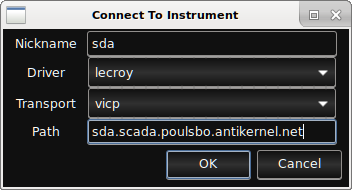
\includegraphics[width=6cm]{images/connection-dialog.png}
\caption{Connection dialog}
\label{connection-dialog}
\end{figure}

It is also possible to connect to arbitrarily many instruments by passing the ``connection string" for each instrument
as a command-line argument.

\begin{lstlisting}[language=sh]
./glscopeclient --debug \
	mylecroy:lecroy:vicp:myscope.example.com:1234 \
	myrigol:rigol:lan:rigol.example.com
\end{lstlisting}

The \texttt{--debug} argument may be omitted or replaced with any other liblogtools argument for controlling console
debug verbosity (\texttt{--quiet}, \texttt{--verbose}, \texttt{--debug}, \texttt{--trace}, etc). If you're using
glscopeclient at its current level of maturity you're probably a developer, so we suggest \texttt{--debug} by default.

Each instrument is described by a ``connection string" containing four colon-separated fields.

\begin{itemize}
\item Nickname. This can be any text string not containing spaces or colons. If you have only one instrument it's
largely ignored, but when multiple instruments are present channel names in the UI are prefixed with the nickname to
avoid ambiguity.
\item Driver name. This is a string identifying the command protocol the scope uses. Note that not all
scopes from the same vendor will use the same command set or driver!
\item Transport. This is is a string describing how the driver connects to the scope (e.g. RS232 or Ethernet)
\item Arguments for the driver identifying the device to connect to, separated by colons. This varies by driver but is
typically a hostname:port combination, TTY device path, or similar.
\end{itemize}

\section{Design Philosophy}

glscopeclient's UI is heavily mouse driven and context based. Space used by always-visible buttons, sliders, etc is
kept to a minimum in order to keep as much screen real estate as possible usable for waveform display. Additional
controls are displayed in menus or pop-up dialogs, then hidden as soon as they are not needed.

Most UI elements can be interacted with by left clicking (select), left dragging (move), using the scroll wheel (zoom),
double clicking (open properties dialog), or right clicking (context menu).

\chapter{Transports}
\label{sec:transports}

\section{gpib}

SCPI over GPIB.

This transport takes up to four arguments: GPIB board index, primary address, secondary address, and timeout value.
Only board index and primary address are required.

NOTE: The current implementation of this driver only works on Linux, using the linux-gpib library.

Example:
\begin{lstlisting}[language=sh, numbers=none]
glscopeclient myscope:keysightdca:gpib:0:7
\end{lstlisting}

\section{lan}

SCPI over TCP with no further encapsulation.

This transport takes two arguments: hostname/IP and port number.

If port number is not specified, uses TCP port 5025 (IANA assigned) by default. Note that Rigol oscilloscopes use the
non-standard port 5555, not 5025, so the port number must always be specified when using a Rigol instrument.

Example:
\begin{lstlisting}[language=sh, numbers=none]
glscopeclient myscope:rigol:lan:192.0.2.9:5555
\end{lstlisting}

\section{lxi}

SCPI over LXI VXI-11.

Note that due to the remote procedure call paradigm used by LXI, it is not possible to batch multiple outstanding
requests to an instrument when using this transport. Some instruments may experience reduced performance when using LXI
as the transport.

Example:
\begin{lstlisting}[language=sh, numbers=none]
glscopeclient myscope:tektronix:lxi:192.0.2.9
\end{lstlisting}

\section{null}

This transport does nothing, and is used as a placeholder for development simulations or non-SCPI instruments.

NOTE: Due to limitations of the current command line argument parsing code, an argument must be provided to all transports,
including this one. Since the argument is ignored, any non-empty string may be used.

Example:
\begin{lstlisting}[language=sh, numbers=none]
glscopeclient sim:demo:null:blah
\end{lstlisting}

\section{twinlan}

This transport is used by some Antikernel Labs oscilloscopes, as well as most of the bridge servers used for interfacing
libscopehal with USB oscilloscopes' SDKs. It takes three arguments: hostname/IP and two port numbers.

It uses two TCP sockets on different ports. The first carries SCPI text (as in the ``lan" transport), and the second is
for binary waveform data.

If port numbers are not specified, the SCPI port defaults to the IANA standard of 5025, and the data port defaults to
5026. If the SCPI port but not the data port is specified, the data port defaults to the SCPI port plus one.

\section{uart}

SCPI over RS-232 or USB-UART.

This transport takes two arguments: device path (required) and baud rate (optional). If baud rate is not specified, it
defaults to 115200.

Example:
\begin{lstlisting}[language=sh, numbers=none]
glscopeclient myscope:rigol:uart:/dev/ttyUSB0:115200
\end{lstlisting}

\section{usbtmc}

SCPI over USB Test \& Measurement Class protocol.

This transport takes one argument: the path to the usbtmc kernel device object.

NOTE: The current implementation of this driver only works on Linux. There is currently no support for USBTMC on
Windows (see scopehal:301)

Example:
\begin{lstlisting}[language=sh, numbers=none]
glscopeclient myscope:siglent:usbtmc:/dev/usbtmc0
\end{lstlisting}

\section{vicp}

SCPI over Teledyne LeCroy Virtual Instrument Control Protocol.

This transport takes two arguments: hostname/IP and port number.

If port number is not specified, uses TCP port 1861 (IANA assigned) by default.

Example:
\begin{lstlisting}[language=sh, numbers=none]
glscopeclient myscope:lecroy:vicp:192.0.2.9
\end{lstlisting}



\section{Oscilloscope Drivers}
\label{sec:drivers}

\subsection{Agilent}

Agilent devices support a similar similar SCPI command set across most device families.

Please see the table below for details of current hardware support:

\begin{tabularx}{16cm}{llX}
\thickhline
\textbf{Device Family} & \textbf{Driver} & \textbf{Notes} \\
\thickhline
DSO5000 series & agilent & Not recently tested, but should work.\\
\thickhline
DSO6000 \& MSO6000 series & agilent &  Working. No support for digital channels yet.\\
\thickhline
DSO7000 \& MSO7000 series & agilent &  Untested, but should work. No support for digital channels yet.\\
\thickhline
\end{tabularx}

\subsubsection{agilent}

Example:
\begin{lstlisting}[language=sh]
./glscopeclient --debug myscope:agilent:lan:192.168.1.1:5025
\end{lstlisting}

This driver has been tested on an MSO6034A.

\subsection{Antikernel Labs}

\begin{tabularx}{16cm}{llX}
\thickhline
\textbf{Device Family} & \textbf{Driver} & \textbf{Notes} \\
\thickhline
Internal Logic Analyzer IP & akila & \\
\thickhline
BLONDEL Oscilloscope Prototype & aklabs & \\
\thickhline
\end{tabularx}

\subsubsection{akila}

This driver uses a raw binary protocol, not SCPI.

Under-development internal logic analyzer analyzer core for FPGA design debug. The ILA uses a UART interface to a host
system. Since there's no UART support in scopehal yet, socat must be used to bridge the UART to a TCP socket using
the ``lan" transport.

\subsubsection{aklabs}

This driver uses two TCP sockets. Port 5025 is used for SCPI control plane traffic, and port 50101 is used for waveform
data using a raw binary protocol.

\subsection{Enjoy Digital}
TODO (scopehal:79)

\subsection{Hantek}
TODO (scopehal:26)

\subsection{Keysight}
TODO

\subsection{Pico Technologies}
TODO (scopehal:15)

\subsection{Rigol}

Rigol oscilloscopes have subtle differences in SCPI command set, but this is implemented with quirks handling in the
driver rather than needing different drivers for each scope family.

\begin{tabularx}{16cm}{llX}
\thickhline
\textbf{Device Family} & \textbf{Driver} & \textbf{Notes} \\
\thickhline
DS1000Z & rigol & \\
\thickhline
MSO5000 & rigol & \\
\thickhline
\end{tabularx}

\subsubsection{rigol}

This driver has been primarily tested on a MSO5000 series scope.

\subsection{Rohde \& Schwarz}
TODO (scopehal:59)

\subsection{Saleae}
TODO (scopehal:16)

\subsection{Siglent}

Many recent Siglent oscilloscopes are developed in partnership with Teledyne LeCroy (Siglent-designed hardware running
Teledyne LeCroy firmware) and are sold under both brands. As a result, there is some crossover in driver support. \\

\begin{tabularx}{16cm}{llX}
\thickhline
\textbf{Device Family} & \textbf{Driver} & \textbf{Transport} & \textbf{Notes} \\
\thickhline
SDS5000X series & siglent & lxi, lan & Untested \\
\thickhline
SDS2000X Plus series & siglent & lxi, lan & Untested \\
\thickhline
SDS2000X-E series & siglent & lxi, lan & Untested \\
\thickhline
SDS2000X series & siglent & lxi & Base functionality present, tested on SDS2304X. \\
\thickhline
SDS1000X series & siglent & lxi & Untested \\
\thickhline
SDS1000X+ series & siglent & lxi & Untested \\
\thickhline
SDS1000X-E series & siglent & lxi, lan & Base functionality present, lan transport tested on SDS1204X-E.\\
\thickhline
SDS1000CFL series & siglent & ? & Untested \\
\thickhline
SDS1000DL+ series & siglent & lxi & Untested \\
\thickhline
SDS1000CML+ series & siglent & lxi & Untested \\
\thickhline
SDS3000X series & lecroy & vicp & Should be same as WaveSurfer 3000 \\
\end{tabularx}

Unlike TCP/IP sockets (``lan"), VXI-11 (``lxi") is a synchronous protocol that  does not support
queueing multiple transactions. When an oscilloscope supports both the lan and the lxi transport,
chances are that the lan transport will have a better performance than the lxi transport.

\subsection{Teledyne LeCroy / LeCroy}

Teledyne LeCroy (and older LeCroy) devices use the same driver, but two different transports for LAN connections.

While all Teledyne LeCroy / LeCroy devices use almost identical SCPI command sets, Windows based devices running
XStream or MAUI use a custom framing protocol (``vicp") around the SCPI data while the lower end RTOS based devices use
raw SCPI over TCP (``lan"). Some of these devices also require use of the Siglent driver as they are Siglent OEM
designs rebranded by Teledyne LeCroy and have some quirks in the firmware which require workarounds.

Please see the table below for details on which configuration to use with  your hardware.

\begin{tabularx}{16cm}{lllX}
\thickhline
\textbf{Device Family} & \textbf{Driver} & \textbf{Transport} & \textbf{Notes} \\
\thickhline
DDA & lecroy & vicp & \\
\thickhline
HDO & lecroy & vicp & \\
\thickhline
LabMaster & lecroy & vicp & Untested, but should work\\
\thickhline
MDA & lecroy & vicp & Untested, but should work\\
\thickhline
SDA & lecroy & vicp & Untested, but should work\\
\thickhline
T3DSO & siglent & lan & Untested, but should work\\
\thickhline
WaveAce & siglent & lan & Untested, but should work \\
\thickhline
WaveJet & siglent & lan & Untested, but should work \\
\thickhline
WaveMaster & lecroy & vicp & Untested, but should work \\
\thickhline
WaveRunner & lecroy & vicp & \\
\thickhline
WaveSurfer & lecroy & vicp & \\
\thickhline
\end{tabularx}

\subsubsection{lecroy}

This is the primary driver for MAUI based Teledyne LeCroy / LeCroy devices.

Example:
\begin{lstlisting}[language=sh]
./glscopeclient --debug myscope:lecroy:vicp:192.168.1.1:1861
\end{lstlisting}

This driver has been tested on a wide range of Teledyne LeCroy / LeCroy hardware including DDA 5005, DDA 5005A,
WaveSurfer 3034, WaveRunner 8104, and HDO9204. It should be compatible with any Teledyne LeCroy or LeCroy oscilloscope
running Windows XP or newer and the MAUI or XStream software.

\subsection{Tektronix}
TODO (scopehal:73, scopehal:13)

\subsection{Xilinx}
TODO (scopehal:40)

\chapter{Main Window}

The main window of glscopeclient consists of the menu bar and tool bar at top and a status bar at the bottom. All
remaining space is occupied by one or more waveform groups.

\section{Menu}

\subsection{File}

This menu contains commands for manipulating glscopeclient session files.

A session consists of a YAML file called filename.scopesession containing instrument and UI configuration, as well
as a directory called filename\_data which contains waveform metadata and sample values for all enabled instrument
channels.

\textbf{Save}: The UI layout may be saved to a session file so that a common instrument setup can be returned to in the
future. Waveform data may optionally be saved in the session as well.

\textbf{Open}: Loads a .scopesession file. Checkboxes at the bottom of the file browser dialog allow the UI
configuration, instrument settings, and waveform data to be individually loaded or ignored.

\textbf{Quit}: Exits the application

\subsection{Setup}

\textbf{Instrument Sync}: Synchronizes two or more instruments under a single glscopeclient instance. TODO: more
complete documentation

\textbf{Trigger}: Configures trigger settings

\textbf{Halt Conditions}: Makes glscopeclient pause when a waveform meeting certain conditions is acquired

\subsection{View}

This menu allows display settings to be configured. As of now, the only option is selection of the color palette for
eye patterns.

\begin{tabularx}{16cm}{llX}
\thickhline
\textbf{Name} & \textbf{Colors} & \textbf{Notes} \\
\thickhline
CRT & 
\includegraphics[width=5cm]{images/eye-gradient-crt.png} & Similar color scheme to a major scope vendor.\\
Grayscale & 
\includegraphics[width=5cm]{images/eye-gradient-grayscale.png} & Common monochrome palette.\\
Ironbow & 
\includegraphics[width=5cm]{images/eye-gradient-ironbow.png} & Common "hot metal" palette. \\
KRain & 
\includegraphics[width=5cm]{images/eye-gradient-krain.png} & Similar color scheme to a major scope vendor.\\
Rainbow & 
\includegraphics[width=5cm]{images/eye-gradient-rainbow.png} & Common HSV rainbow palette. \\
Viridis & 
\includegraphics[width=5cm]{images/eye-gradient-viridis.png} & Perceptually uniform palette from matplotlib. \\
\thickhline
\end{tabularx}

\subsection{Add}

This menu allows a new waveform view to be created for any channel on a connected instrument.

\subsection{Window}

This menu provides access to pop-up windows such as protocol analyzers which were closed.

\subsection{Help}

\textbf{About}: Displays program version and copyright information

\section{Toolbar}

The toolbar contains buttons and controls for the most frequently used actions.

\begin{figure}[h]
\centering

\includegraphics[width=16cm]{images/toolbar.png}
\caption{glscopeclient toolbar}
\label{toolbar}
\end{figure}

\subsection{Capture buttons}

The capture button group (Fig. \ref{capturebuttons}) contains three buttons. From left to right these are ``arm
normal trigger", ``arm one-shot trigger" and ``stop trigger".

Note that the ``normal" trigger mode still uses one-shot capture internally so that all waveform data can be downloaded
before the next trigger event.

\begin{figure}[h]
\centering

\includegraphics[height=1cm]{images/capture-icons.png}
\caption{Capture control buttons}
\label{capturebuttons}
\end{figure}

\subsection{History}

The history button (Fig. \ref{historybutton}) toggles display of the \hyperref[sec:history]{waveform history view}.

\begin{figure}[h]
\centering

\includegraphics[height=1cm]{images/history-button.png}
\caption{History button}
\label{historybutton}
\end{figure}

\subsection{Refresh Settings}

In order to improve performance, glscopeclient caches many instrument settings locally rather than constantly querying
the instrument for the current timebase, trigger configuration, etc. If settings are changed on the instrument while
glscopeclient is running, glscopeclient may not be aware of these changes.

The Refresh Settings button (Fig. \ref{refreshbutton}) clears all cached instrument configuration and updates
glscopeclient with the current instrument settings.

\begin{figure}[h]
\centering

\includegraphics[height=1cm]{images/refresh-button.png}
\caption{Refresh Settings button}
\label{refreshbutton}
\end{figure}

\subsection{Clear Sweeps}

The Clear Sweeps button (Fig. \ref{clearbutton}) clears all persistence waveforms, accumulated eye pattern / waterfall
data, and statistics. Waveforms saved in history are not deleted.

\begin{figure}[h]
\centering

\includegraphics[height=1cm]{images/clear-button.png}
\caption{Clear Sweeps button}
\label{clearbutton}
\end{figure}

\subsection{Fullscreen}

The Fullscreen button (Fig. \ref{fullscreenbutton}) switches glscopeclient between normal and full-screen mode.

\begin{figure}[h]
\centering

\includegraphics[height=1cm]{images/fullscreen-button.png}
\caption{Fullscreen button}
\label{fullscreenbutton}
\end{figure}

\subsection{Opacity slider}

The opacity slider (Fig. \ref{opacityslider}) controls the alpha/opacity used to display intensity-graded waveforms.
Higher opacity values lead to better display of sparse waveforms (compare the crisp lines of Fig. \ref{sparse-waveform}
to the barely visible trace in Fig. \ref{dim-waveform}) but can lead to a washed-out appearance if too many sample
points are shoved into a small area.

\begin{figure}[H]
\centering

\includegraphics[height=1cm]{images/opacity-slider.png}
\caption{Trace opacity slider}
\label{opacityslider}
\end{figure}

\begin{figure}[H]
\centering
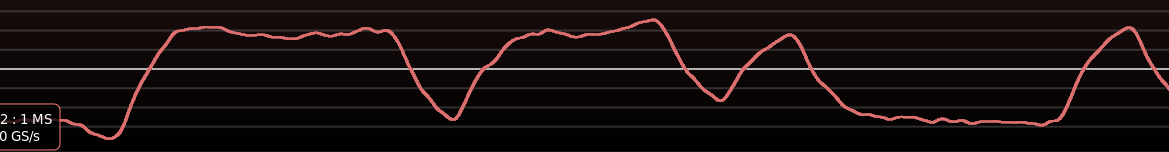
\includegraphics[width=10cm]{images/sparse-waveform.png}
\caption{Sparse waveform at a high zoom level}
\label{sparse-waveform}
\end{figure}

\begin{figure}[H]
\centering
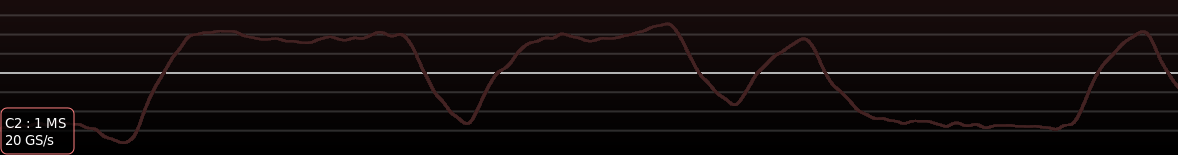
\includegraphics[width=10cm]{images/dim-waveform.png}
\caption{Dim waveform showing difficulty of seeing waveform at low opacity}
\label{dim-waveform}
\end{figure}

For example, the DVI waveform in Fig. \ref{washedout-waveform} looks like a solid white blob with a vaguely visible
outline. No fine detail can be observed other than the increased over/undershoot and random-looking edges on the
scanlines, compared to the flat appearance of the blanking period between scanlines and at the end of the frame.

When the opacity is reduced in this example, many more nuances of the signal become apparent. The high/low voltage
levels of the signal compared to the transitions between them are obvious, and the H/V sync pulses within the blanking
period show up as a slightly darker region.

\begin{figure}[H]
\centering
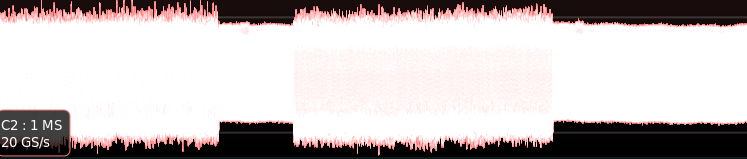
\includegraphics[width=10cm]{images/washedout-waveform.png}
\caption{Intensity-graded waveform showing washed-out appearance at high opacity}
\label{washedout-waveform}
\end{figure}

\begin{figure}[H]
\centering
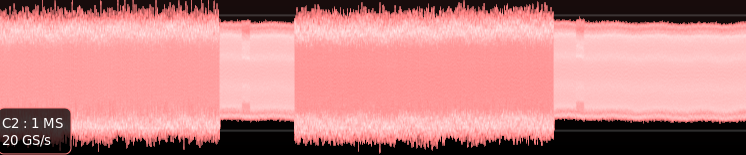
\includegraphics[width=10cm]{images/graded-waveform.png}
\caption{Intensity-graded waveform at lower opacity level}
\label{graded-waveform}
\end{figure}

As of this writing, the opacity setting is global for the entire application. Should this be changed to per waveform
group? If so, how should the group be selected and should there still be an option to make changes globally?

\FloatBarrier
\section{Waveform Groups}

A waveform group is a collection of one or more waveforms stacked vertically under a common timeline. All waveforms
within a group share the same timeline and vertical cursor(s).

When glscopeclient starts up, by default all channels on the attached instruments are displayed in a single waveform
group (Figure \ref{single-group}).

\begin{figure}[h]
\centering
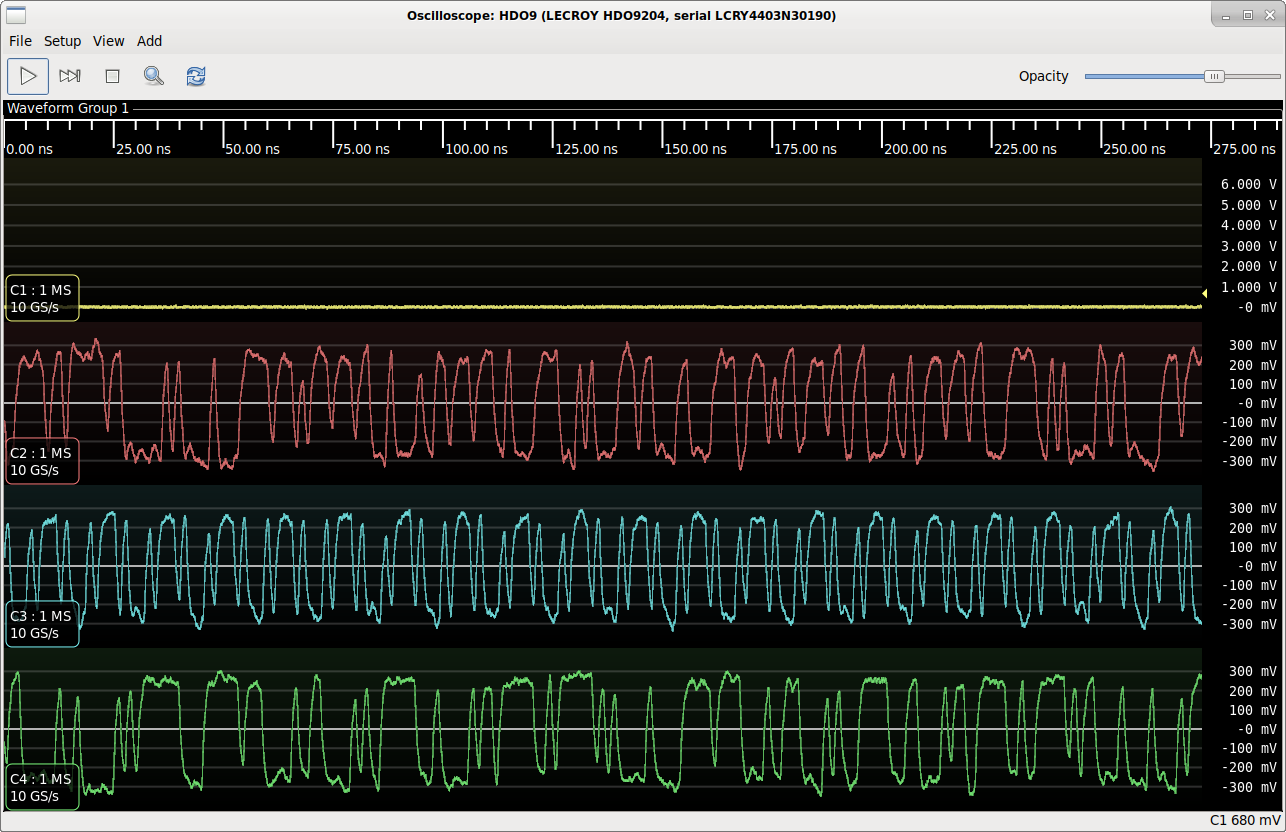
\includegraphics[width=13cm]{images/overview.png}
\caption{Top level glscopeclient window with a single waveform group}
\label{single-group}
\end{figure}

As you add protocol decodes or look at different parts of a waveform, it may be necessary to create additional waveform
groups. Typical reasons for creating additional groups include:

\begin{itemize}
\item Zooming into one set of signals to see detail on short time scales while maintaining a high level overview of
others
\item Viewing signals with incompatible horizontal units. For example, a FFT has horizontal units of frequency while an
analog waveform has horizontal units of time. Eye patterns also have horizontal units of time, but are always displayed
as two UIs wide and cannot be zoomed.
\footnote
{
It is currently possible to place signals with incompatible horizontal units in the same group. This may lead to
confusion; a future software release will likely force creation of a new group if a protocol decode is incompatible
with the parent trace's time scale.
}
\end{itemize}

\subsection{Managing Groups}

Additional groups may be created by right clicking a waveform and selecting \menustyle{[Move|Copy] waveform to / Insert
new group at [right|bottom]} from the context menu. This will split the current group's area in half horizontally or
vertically, with the selected waveform moved or copied to the newly added group and all other waveforms in the original
group.

Waveforms may be also be moved within, or between, groups by clicking the channel information box and dragging it. A
yellow insertion bar will appear when dragging, showing the location the waveform will be inserted in.

If a waveform is dragged to the very bottom or right side of a waveform group, the destination group will be split
vertically or horizontally and the new waveform will be inserted below or to the right of the destination group. The
insertion bar turns orange when dragging near the edge of a group, to indicate that a split will take place.

Dividers between waveform groups may be dragged with the left mouse button. Any group may be subdivided again, to
create arbitrarily complex tiles of waveforms. Figure \ref{multiple-groups} shows a two-level hierarchy created by
moving channel 2 to a new group at right, then moving channel 4 to a new group below that one.

\begin{figure}[h]
\centering
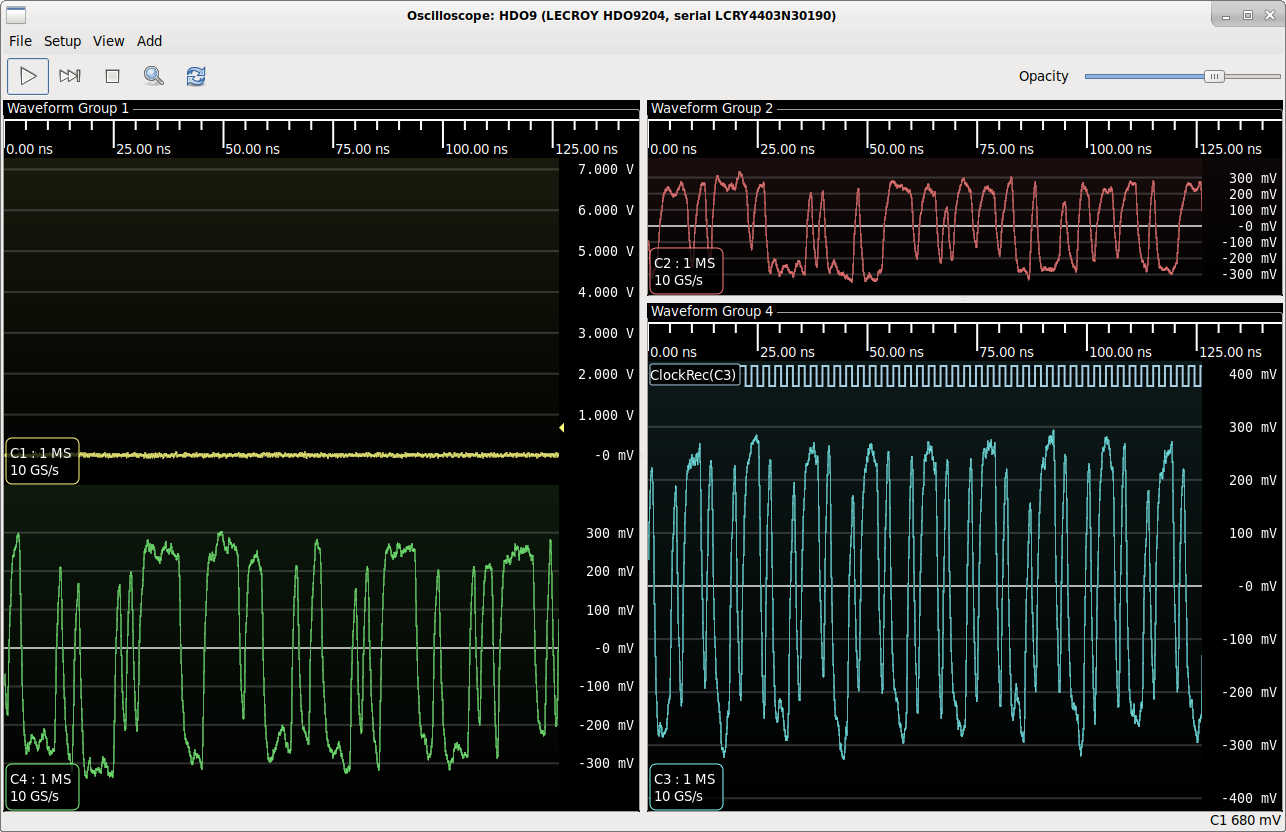
\includegraphics[width=14cm]{images/multiple-groups.png}
\caption{Top level glscopeclient window with several waveform groups separated by splitters}
\label{multiple-groups}
\end{figure}

Protocol decode overlays may be reordered by dragging the channel information box with the mouse, however they cannot
currently be moved to another waveform or group.

New waveform groups are given an automatically generated name when created, for example "Waveform Group 2". This name
will be editable in a future software release (scopehal-apps:53).

\pagebreak
\section{Timeline}

The timeline is displayed at the top of each waveform group and shows the X axis scale for the group. The timeline (and
all accompanying waveform views in the group) may be zoomed by scrolling with the mouse wheel, or panned by dragging
with the left mouse button.

Unlike classical oscilloscope user interfaces, there is \emph{no relationship} between the timeline scale/position and
the duration of the acquisition. It is possible to zoom or scroll beyond the end of the acquisition (displaying empty
background with no signal) or have a deep capture in which nearly all acquired data is offscreen.

TODO: talk about how to set trigger offset in capture and change timebase once that's implemented

TODO: insert screenshot after we have some pending UI changes done

\pagebreak
\section{Waveform Views}

A waveform view is a 2D graph of a signal or protocol decode within a waveform group.

\subsection{Plot Area}

The plot area shows the waveform being displayed. The background has a subtle gradient from light at top to dark at
bottom, in order to visually separate adjacent waveform view within the same group.

The horizontal grid lines line up with the voltage scale markings on the Y axis. If the plot area includes Y=0, the
grid line for zero is slightly brighter.

\begin{figure}[H]
\centering
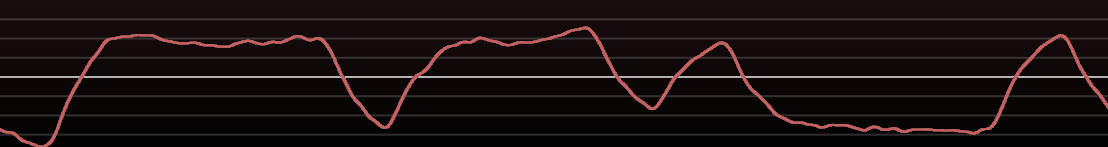
\includegraphics[width=10cm]{images/waveform-graph.png}
\caption{Waveform plot area}
\label{waveform-graph}
\end{figure}

The waveform is drawn as a semi-transparent line so that when zoomed out, the density of voltage at various points in
the graph may be seen as lighter or darker areas. This is referred to as ``intensity grading".

\begin{figure}[H]
\centering
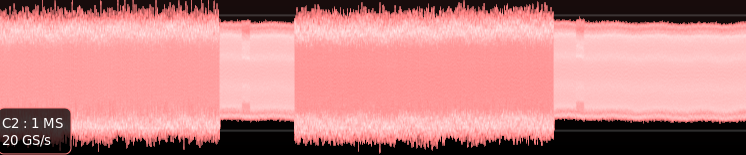
\includegraphics[width=10cm]{images/graded-waveform.png}
\caption{Intensity-graded waveform}
\label{graded-waveform2}
\end{figure}

\subsection{Y Axis Scale}

Each waveform view has its own Y axis scale, which is locked to the ADC range of the instrument.

Dragging the Y axis scale with the left mouse button currently does nothing (scopehal-apps:54) but in a future software
release will change the voltage offset of the channel.

Scrolling the Y axis scale with the mouse wheel changes the gain of the channel.

If a left-pointing arrow (as seen in Fig. \ref{y-axis}) is visible, the current channel is selected as a trigger
source. Click on the arrow and drag up or down to select the trigger level.

\begin{figure}[H]
\centering
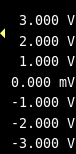
\includegraphics[height=3cm]{images/y-axis.png}
\caption{Y axis of a waveform view showing trigger arrow}
\label{y-axis}
\end{figure}

\subsection{Channel Information Box}

The channel information box is displayed in the lower left corner of each waveform view. It contains summary
information about the channel. Currently this is the display name of the channel, the sample rate, and the record
length of the acquisition. Other information, such as probe coupling, may be displayed there in the future.

Double-clicking the information box opens the channel properties dialog.

\begin{figure}[H]
\centering
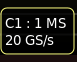
\includegraphics[width=2cm]{images/channel-infobox.png}
\caption{Channel information box}
\label{channel-infobox}
\end{figure}

\subsection{Overlays}

Waveforms may have additional information overlaid on top of them, such as protocol decodes. Each overlay has its own
information box, which may be double-clicked to open the properties dialog and configure it just like any other
channel.

Fig. \ref{overlays} shows
an example of an analog waveform with three overlays: thresholding it to NRZ digital, recovering a sampling
clock with a CDR PLL, and finally decoding the serial NRZ data stream to TMDS protocol data and control events.

\begin{figure}[H]
\centering
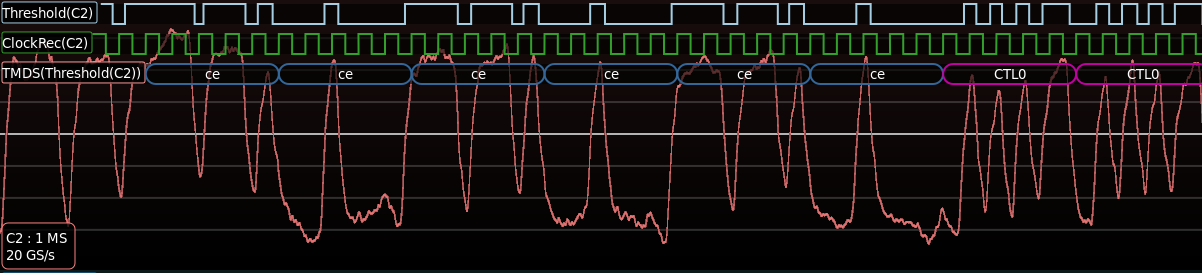
\includegraphics[width=14cm]{images/overlays.png}
\caption{Waveform showing two digital overlays and a data decode overlay}
\label{overlays}
\end{figure}

Overlays can be deleted but cannot currently be moved between waveform areas or reordered within a single waveform area
(scopehal-apps:7, scopehal-apps:6)

\chapter{Timeline}

The timeline is displayed at the top of each waveform group and shows the X axis scale for the group. The timeline (and
all accompanying waveform views in the group) may be zoomed by scrolling with the mouse wheel, or panned by dragging
with the left mouse button.

Unlike classical oscilloscope user interfaces, there is \emph{no relationship} between the timeline scale or position
and the duration of the acquisition. It is possible to zoom or scroll beyond the end of the acquisition (displaying
empty background with no signal) or have a deep capture in which nearly all acquired data is offscreen.

Note that the timeline may occasionally show units other than time. For example, an ``eye width" measurement has X axis
units of voltage and Y axis units of time, and a spectrum analyzer channel has X axis units of frequency.


\begin{figure}[h]
\centering
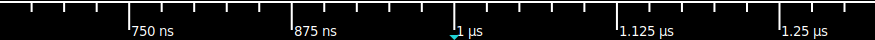
\includegraphics[width=14cm]{images/timeline.png}
\caption{The timeline}
\label{timeline}
\end{figure}

The position of the trigger event is marked by a downward-pointing arrow on the timeline, color coded to match the
channel selected as the primary trigger source. The trigger arrow cannot be interacted with currently, but in the future
(scopehal-apps:173) it will be draggable to adjust the trigger position.

Double-clicking on the timeline brings up the timebase properties dialog (Fig. \ref{timebase-properties}), which allows
the sample rate and memory depth to be configured. If multiple instruments are connected, a separate tab appears in the
dialog for each instrument.

\begin{figure}[h]
\centering
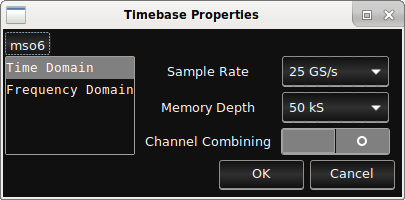
\includegraphics[width=9cm]{images/timebase-properties.png}
\caption{Timebase properties (time domain)}
\label{timebase-properties}
\end{figure}

If the instrument is a spectrum analyzer, or has frequency-domain analysis capability (such as the Tektronix MSO5 and
MSO6 oscilloscopes), the timebase properties dialog will have a second page (Fig. \ref{timebase-properties-freq}) for
setting the span and resolution bandwidth for frequency-domain channels. Center frequency is often a per-channel
adjustment, so it is configured from the channel properties dialog rather than timebase properties.

\begin{figure}[h]
\centering
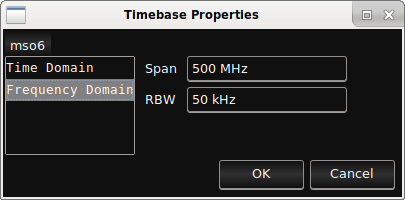
\includegraphics[width=9cm]{images/timebase-properties-freq.png}
\caption{Timebase properties (frequency domain)}
\label{timebase-properties-freq}
\end{figure}

\chapter{Triggers}

\section{Trigger Properties}

The \menustyle{Setup / Trigger} menu opens the trigger properties dialog (Fig. \ref{trigger-properties}).

The Trigger Type box allows the type of trigger to be chosen. The list of available triggers depends on the instrument
model and installed software options.

The Trigger Offset field specifies the time from the \emph{start} of the waveform to the trigger point. Positive values
move the trigger later into the waveform, negative values introduce a delay between the trigger and the start of the
waveform. \footnote{This is a different convention than most oscilloscopes, which measure the trigger position from the
\emph{midpoint} of the waveform. Since glscopeclient decouples the acquisition length from the UI zoom setting,
measuring from the midpoint makes little sense as there are no obvious visual cues to the midpoint's location.}

\begin{figure}[h]
\centering
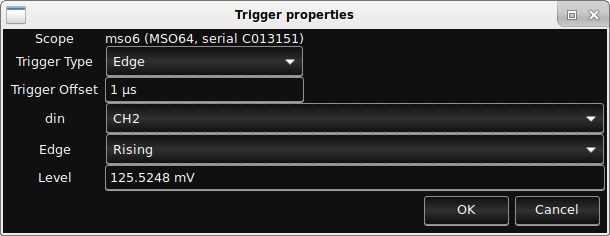
\includegraphics[width=9cm]{images/trigger-properties.png}
\caption{Trigger properties dialog}
\label{trigger-properties}
\end{figure}

The remaining settings in the trigger properties dialog depend on the specific trigger type chosen.

\section{Dropout}

Triggers when a signal stops toggling for a specified amount of time.

\section{Edge}

Triggers on edges in the signal.

\section{Pulse Width}

Triggers when a high or low pulse meeting specified width criteria is seen.

\section{Runt}

Triggers when a pulse crosses one threshold, but not a second.

\section{Slew Rate}

Triggers when an edge is faster or slower than a specified rate.

\section{UART}

Triggers when a byte or byte sequence is seen on a UART.

\section{Window}

Triggers when a signal goes above or below specified thresholds.

\chapter{Waveform Views}

A waveform view is a 2D graph of a signal or protocol decode within a waveform group.

\section{Navigation}

Scrolling with the mouse wheel adjusts the horizontal scale of the current waveform group, zooming in or out centered
on the position of the mouse cursor.

Pressing SHIFT while scrolling moves the view left and right without adjusting zoom. If your mouse has a horizontal
scroll feature, this may also be used to pan without zooming.

\section{Plot Area}

The plot area shows the waveform being displayed. The background has a subtle gradient from light at top to dark at
bottom, in order to visually separate adjacent waveform view within the same group.

The horizontal grid lines line up with the voltage scale markings on the Y axis. If the plot area includes Y=0, the
grid line for zero is slightly brighter.

\begin{figure}[H]
\centering
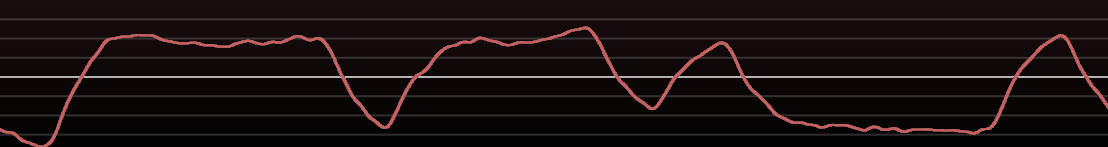
\includegraphics[width=10cm]{images/waveform-graph.png}
\caption{Waveform plot area}
\label{waveform-graph}
\end{figure}

The waveform is drawn as a semi-transparent line so that when zoomed out, the density of voltage at various points in
the graph may be seen as lighter or darker areas. This is referred to as ``intensity grading".

\begin{figure}[H]
\centering
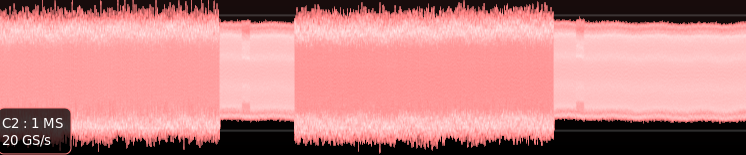
\includegraphics[width=10cm]{images/graded-waveform.png}
\caption{Intensity-graded waveform}
\label{graded-waveform2}
\end{figure}

\section{Y Axis Scale}

Each waveform view has its own Y axis scale, which is locked to the ADC range of the instrument.

If the waveform view is connected to a physical channel of an instrument, the gain may be configured by scrolling with
the mouse wheel, and the offset may be adjusted by dragging with the left mouse button. If the view is displaying the
output of a filter block, gain and offset are set by the filter and generally not adjustable, although some (such as
FFTs) do allow adjustment.

If a left-pointing arrow (as seen in Fig. \ref{y-axis}) is visible, the current channel is selected as a trigger
source. Click on the arrow and drag up or down to select the trigger level. Some trigger types, such as window triggers,
have two arrows for upper and lower levels.

\begin{figure}[H]
\centering
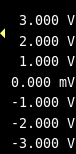
\includegraphics[height=3cm]{images/y-axis.png}
\caption{Y axis of a waveform view showing trigger arrow}
\label{y-axis}
\end{figure}

\section{Channel Information Box}

The channel information box is displayed in the lower left corner of each waveform view. It contains summary
information about the channel. Currently this is the display name of the channel, the sample rate, and the record
length of the acquisition. Other information, such as probe coupling, may be displayed there in the future.

\begin{figure}[H]
\centering
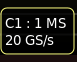
\includegraphics[width=2cm]{images/channel-infobox.png}
\caption{Channel information box}
\label{channel-infobox}
\end{figure}

The information box may be dragged with the left mouse button to move the entire waveform view to a new location.

Double-clicking the information box opens the channel properties dialog (Fig. \ref{channel-properties}). This dialog
allows changing of the channel's nickname or color. The ``hardware name" of the channel is also displayed, so that a
renamed channel can be easily traced back to a physical instrument input.

\begin{figure}[H]
\centering
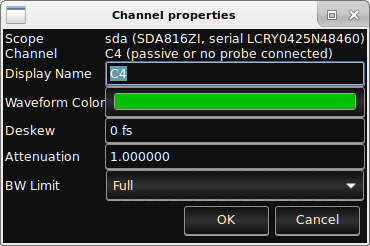
\includegraphics[width=8cm]{images/channel-properties.png}
\caption{Channel properties dialog}
\label{channel-properties}
\end{figure}

\section{Overlays}

Waveforms may have additional information overlaid on top of them, such as protocol decodes. Each overlay has its own
information box, which may be double-clicked to open the properties dialog and configure it just like any other
channel.

Fig. \ref{overlays} shows
an example of an analog waveform with three overlays: thresholding it to NRZ digital, recovering a sampling
clock with a CDR PLL, and finally decoding the serial NRZ data stream to TMDS protocol data and control events.

\begin{figure}[H]
\centering
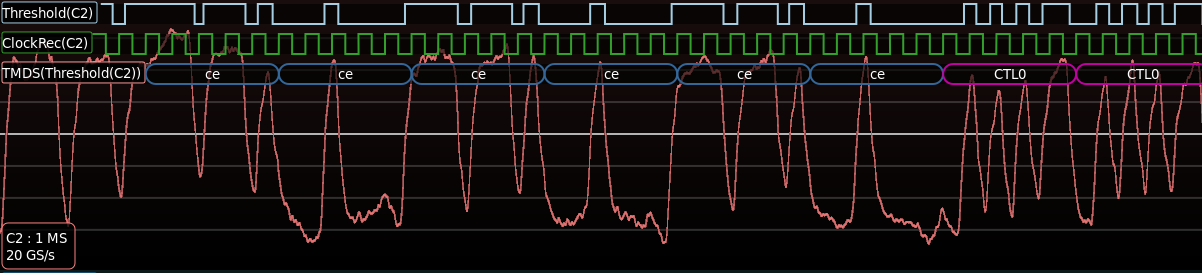
\includegraphics[width=14cm]{images/overlays.png}
\caption{Waveform showing two digital overlays and a data decode overlay}
\label{overlays}
\end{figure}

Overlays can be deleted by means of the right-click context menu. Dragging the information box with the left mouse
button allows overlays to be reordered, however they cannot currently be moved to another waveform view.

\section{Statistics}

Statistics may be shown for any waveform by checking the ``statistics" box in the context menu. The default statistics
are minimum, average, and maximum although more may be added in the future.

\chapter{History View}
\label{sec:history}

glscopeclient has the ability to save every waveform during a session in memory, allowing you to go back in time and
see previous state of the system being debugged. Clicking on a timestamp in the history view pauses acquisition and
loads the historical waveform data for analysis.

By default, the history view (Fig. \ref{historyview}) is not displayed and history is limited to ten waveforms. If the
history view is closed, history continues to be captured up to the configured maximum history depth.

\begin{figure}[H]
\centering
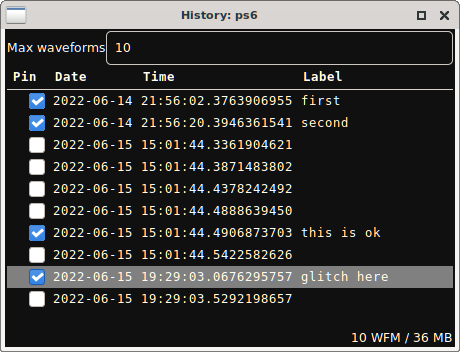
\includegraphics[width=5cm]{images/history-view.png}
\caption{Waveform history view}
\label{historyview}
\end{figure}

The ``max waveforms" box allows the depth of the history to be configured. It defaults to 10 but can be set to any
positive integer value. Older waveforms beyond the history limit are deleted as new waveforms are acquired.

The status bar at the bottom of the history view displays the total number of waveforms in the history, as well as an
estimate of the amount of RAM used by the history.

\section{Estimating Waveform Memory Usage}

When selecting a maximum depth for the history, it is important to pick a reasonable limit to avoid running out of RAM!
glscopeclient will happily fill tens or hundreds of gigabytes of memory with deep waveforms if given a chance. Memory
usage of waveform data can be roughly estimated as 16 + sizeof(sample type) bytes per point, since each sample contains a
64-bit timestamp and duration plus the sample data.

For example, an analog sample takes 20 bytes of RAM (16 of time plus a 32-bit floating point voltage measurement) per
sample. Thus, a 1M point analog waveform takes approximately 20 MB of RAM per channel, or 80 MB per capture on a
four-channel oscilloscope with all channels enabled.

On the larger side, a 10M point four channel capture would use 800 MB and a 64M point deep-memory capture would use 5
GB. A deep history setting, such as 100 waveforms, is thus wildly inappropriate for such deep captures! A future
software release may support spilling waveform data to a temporary directory on disk, permitting effectively unlimited
history depth given sufficient disk space.

Digital waveforms use one byte per sample for the actual measurement, so 17 MB per channel for a 1M point waveform.
Most logic analyzer or MSO drivers for libscopehal will perform automatic de-duplication when a waveform goes several
clock cycles with no toggles, so the actual memory usage is likely to be significantly less than this.

Filter memory usage varies depending on the specific filter in question, however it is typically not a large
contributor to the overall glscopeclient RAM footprint when using history mode because filters are evaluated
dynamically each time a waveform is pulled from history rather than having output cached for every historical waveform.
Thus, at most one copy of each filter's output is present in memory regardless of history depth.

\chapter{Protocol Analyzer View}
\label{chapter:protoanalyzer}

Some filters for decoding packet-oriented data provide an alternate means of visualizing the decoded traffic.

The protocol analyzer view (Fig. \ref{proto-analyzer}) displays each packet in the history as a row in a list view. The
first column is always the timestamp of the packet; remaining columns vary depending on the particular filter in
question.

\begin{figure}[H]
\centering
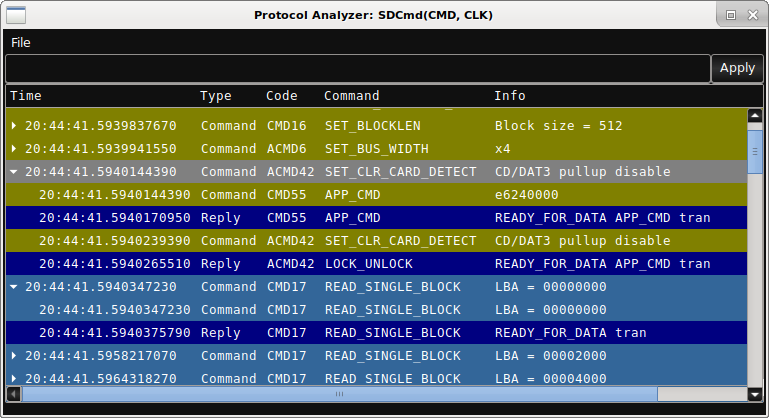
\includegraphics[width=14cm]{images/proto-analyzer.png}
\caption{Protocol analyzer view}
\label{proto-analyzer}
\end{figure}

If closed, the protocol analyzer view may be reopened by selecting the protocol of interest from the
\menustyle{Window / Analyzer} menu.

Many filters group related packets (request and reply, escape sequences, polling loops, etc) under a single heading to
enable easier navigation of large datasets. The tree expansion button at the left of the timestamp column may be used
to expand the event into its constituent packets.

\section{Cursor Interaction}

Clicking on a packet pauses acquisition, loads the relevant waveform from history if the packet is not in the current
waveform, and scrolls the waveform view containing the protocol decode to show the packet. If the packet fits entirely
within the view at the current zoom setting it is centered in the view; otherwise the beginning of the packet is placed
near the left edge of the viewport and the packet continues off the right edge.

If a vertical cursor (Sec. \ref{sec:cursors}) is active in the waveform area displaying the protocol decode, clicking
on a packet in the analyzer view moves the cursor to the start of the packet. Placing the cursor on a packet highlights
the corresponding row in the protocol analyzer.

\section{Packet Coloring}

Protocol packets are color coded according to the high-level function of the packet. The colors are configurable in
preferences; defaults are shown in the table below.

\begin{tabularx}{16cm}{llX}
\thickhline
\textbf{Color name} & \textbf{Use case} & \textbf{Default Color} \\
\thickhline
Command & Executing commands & \cellcolor{protocmd}\textcolor{white}{\#600050} \\
\thickhline
Control & Changing configuration & \cellcolor{protoctl}\textcolor{white}{\#808000} \\
\thickhline
Data read & Reading data & \cellcolor{protoread}\textcolor{white}{\#336699} \\
\thickhline
Data write & Writing data & \cellcolor{protowrite}\textcolor{white}{\#339966} \\
\thickhline
Error & Malformed, bad checksum & \cellcolor{protoerror}\textcolor{white}{\#ff0000} \\
\thickhline
Status & Status updates, flow control & \cellcolor{protostatus}\textcolor{white}{\#000080} \\
\thickhline
\end{tabularx}

\section{Filtering}

To ease analysis of large packet datasets, filters may be applied to the analyzer view by typing a filter expression
into the filter bar at the top of the window (Fig. \ref{proto-filter}), then pressing the ``Apply" button. A filter can
be removed by deleting the contents of the filter bar and pressing ``Apply".

\begin{figure}[H]
\centering
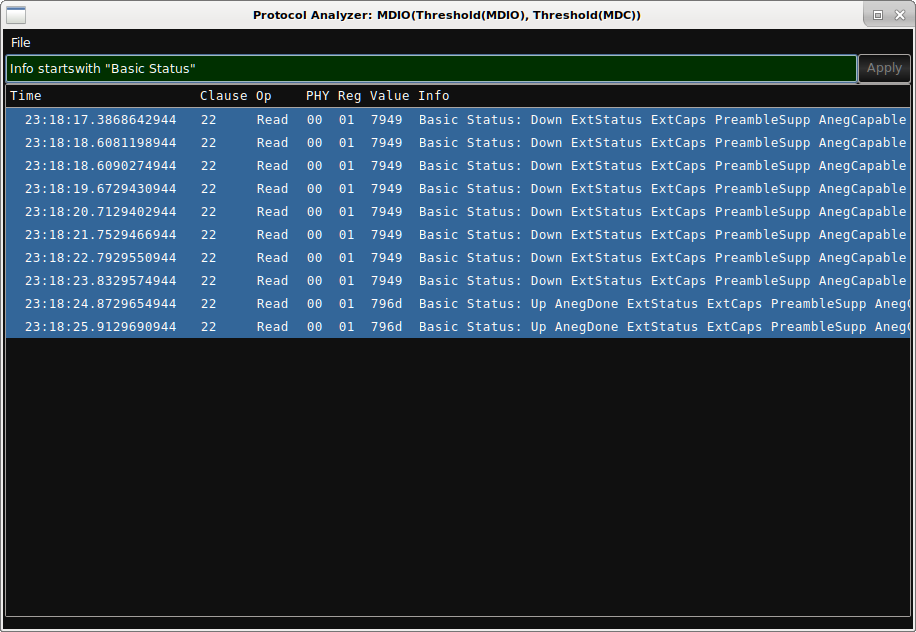
\includegraphics[width=14cm]{images/proto-filter.png}
\caption{Filtering protocol analyzer view}
\label{proto-filter}
\end{figure}

The basic format of a filter is (expression) (operator) (expression).

\subsection{Expressions}

An expression can be:
\begin{itemize}
\item A quoted string
\item A decimal number
\item A field identifier (such as \texttt{PHY} or \texttt{Reg}). Identifiers are case sensitive.
\item data[x], where x is an arbitrary numeric expression
\item A filter expression in parentheses. This expression must evaluate to boolean true or false. The unary ! operator
can be used to negate a parenthetical expression.
\end{itemize}

\subsection{Operators}

An operator can be:
\begin{itemize}
\item \texttt{==}: returns true if the left and right expression are equal
\item \texttt{!=}: returns true if the left and right expression are not equal
\item \texttt{||}: returns true if at least one of the left or right expression is true
\item \texttt{\&\&}: returns true if both the left and right expression is true
\item \texttt{startswith}: returns true if the right expression is a string which starts with the left expression
\item \texttt{contains}: returns true if the right expression is a string which contains the left expression
\end{itemize}

\subsection{Examples of filters}

\begin{lstlisting}[language=C]
Op == "Read"
Reg == "0f"
(Clause == 22) && (Info startswith "Basic Status")
\end{lstlisting}

\chapter{Filter Graph Editor}

The filter graph editor allows complex signal processing pipelines to be developed in a graphical fashion.

It may be accessed from the \menustyle{Window / Filter Graph} menu item.

The leftmost column shows all of the input channels which may be used as data sources for the filter graph. Filter
nodes are automatically placed in columns such that data flows from left to right, with inputs at the left and outputs
at the right of each node.

Nodes may be dragged vertically within their column by using the left mouse button, however the horizontal position of
each node is fixed.

To make a connection, click on the source node's output and then on the destination node's input. To cancel an
in-progress connection, simply click anywhere outside a node.

\begin{figure}[H]
\centering
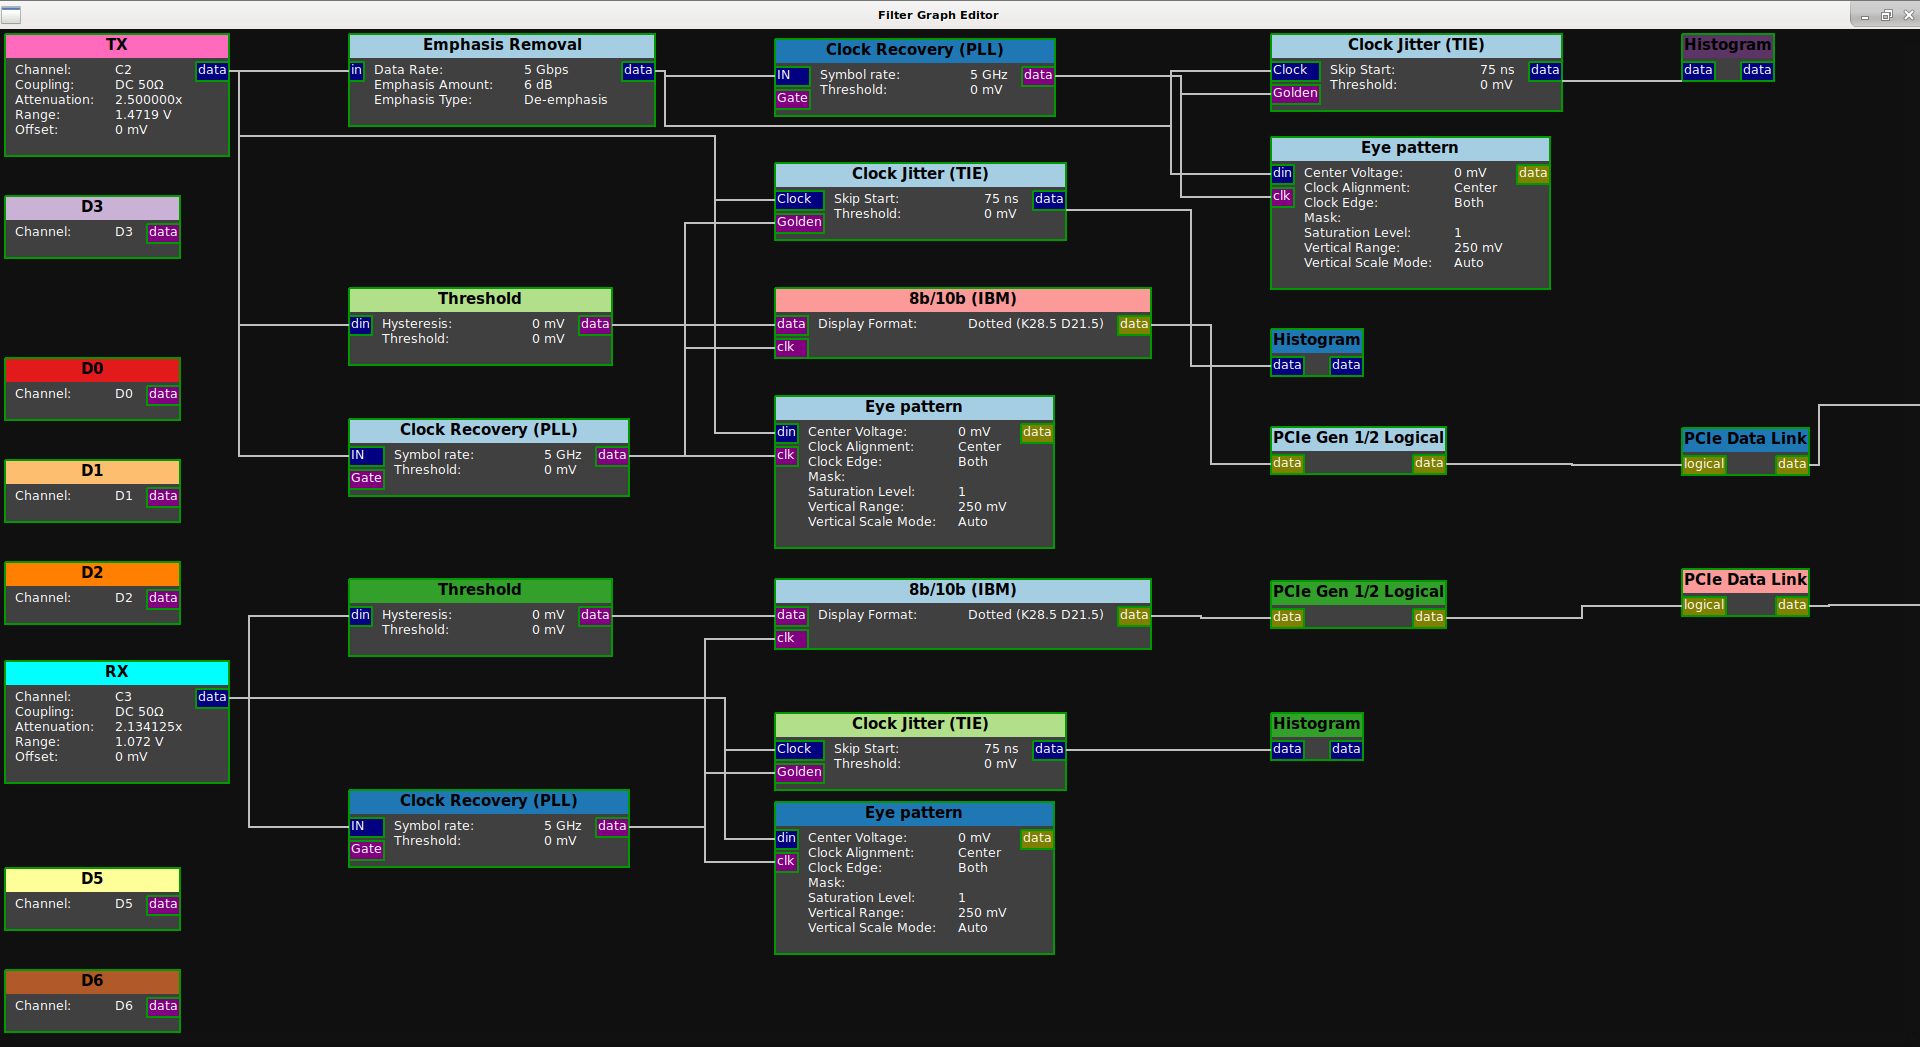
\includegraphics[width=17cm]{images/graph-editor.png}
\caption{Filter graph editor view}
\label{graph-editor}
\end{figure}

The title bar of each node in the graph is color coded to match the channel's color in the waveform view.

Input and output ports are color coded according to the type of data. The colors are configurable under the
\menustyle{Appearance / Filter Graph} preference category; the default assignment is dark blue for analog, purple for
digital, and olive for protocol decodes and other non-primitive types.

\chapter{Filters}

\section{Introduction}

\subsection{Key Concepts}

glscopeclient and libscopehal are based on a ``filter graph" architecture internally. The filter graph is a directed
acyclic graph with a set of source nodes (waveforms captured from hardware or loaded from a saved session) and sink
nodes (waveform views, protocol analyzer views, and statistics) connected by edges representing data flow.

A filter is simply an intermediate node in the graph, which takes input from one or more waveform nodes and outputs a
waveform which may be displayed, used as input to other filters, or both. A waveform is a series of data points which
may represent voltages, digital samples, or arbitrarily complex protocol data structures.

As a result, there is no internal distinction between math functions, measurements, and protocol decodes, and it is
possible to chain them arbitrarily. Consider the following example:

\begin{itemize}
\item Two analog waveforms representing serial data and clock are acquired
\item Each analog waveform is thresholded, producing a digital waveform
\item The two digital waveforms are decoded as $I^2C$, producing a series of packets
\item The $I^2C$ packets are decoded as writes to a serial DAC, producing an analog waveform
\item A moving average filter is applied to the analog waveform
\item A measurement filter finds the instantaneous frequency of each cycle of the DAC output
\end{itemize}

In this document we use the term ``filter" consistently to avoid ambiguity.

\subsection{Conventions}

Each filter takes one or more inputs (vector inputs), zero or more parameters (scalar inputs), and outputs a
signal (vector output).

If the output signal is a complex-valued type (as opposed to a single scalar, e.g. voltage, at each sample) the
``Output Signal" section will include a table describing how various types of output data are displayed. Printf-style
format codes maybe used for clarity. For example, ``\%02x" means data is formatted as hexadecimal bytes with leading
zeroes.

All filters with complex output use a standardized set of colors to display various types of data fields in a
consistent manner. These colors are configurable under the \menustyle{Appearance / Decodes} preferences category.

\begin{tabularx}{16cm}{llX}
\thickhline
\textbf{Color name} & \textbf{Use case} & \textbf{Default Color} \\
\thickhline
Address & Memory addresses & \cellcolor{address}\textcolor{black}{\#ffff00} \\
\thickhline
Checksum Bad & Incorrect CRC/checksum & \cellcolor{checksumbad}\textcolor{white}{\#ff0000} \\
\thickhline
Checksum OK & Valid CRC/checksum & \cellcolor{checksumok}\textcolor{black}{\#00ff00} \\
\thickhline
Control & Miscellaneous control data & \cellcolor{control}\textcolor{white}{\#c000a0} \\
\thickhline
Data & User data & \cellcolor{data}\textcolor{white}{\#336699} \\
\thickhline
Error & Malformed/unreadable data & \cellcolor{error}\textcolor{white}{\#ff0000} \\
\thickhline
Idle & Inter-frame gaps & \cellcolor{idle}\textcolor{white}{\#404040} \\
\thickhline
Preamble & Preamble/sync words & \cellcolor{preamble}\textcolor{white}{\#808080} \\
\thickhline
\end{tabularx}

%%%%%%%%%%%%%%%%%%%%%%%%%%%%%%%%%%%%%%%%%%%%%%%%%%%%%%%%%%%%%%%%%%%%%%%%%%%%%%%%%%%%%%%%%%%%%%%%%%%%%%%%%%%%%%%%%%%%%%%%
\pagebreak
\section{64b/66b}
\label{filter:64b66b}

Decodes the 64/66b line code used by \hyperref[filter:10gbaser]{10Gbase-R} and other serial protocols, as originally
specified in IEEE 802.3 clause 49.2.

64b/66b is a serial line code which divides transmitted data into 64-bit blocks and scrambles them with a LFSR, then
appends a 2-bit type field (which is not scrambled) to each block for synchronization. Block synchronization depends on
always having an edge in the type field so types 2'b00 and 2'b11 are disallowed.

Note that this filter only performs block alignment and descrambling. No decoding is applied to the 64-bit blocks, as
different upper-layer protocols assign different meaning to them. In 10Gbase-R, type 2'b01 denotes ``64 bits of upper
layer data" and type 2'b10 denotes ``8-bit type field and 56 bits of data whose meaning depends on the type", however
this is not universal.

\begin{figure}[h]
\centering
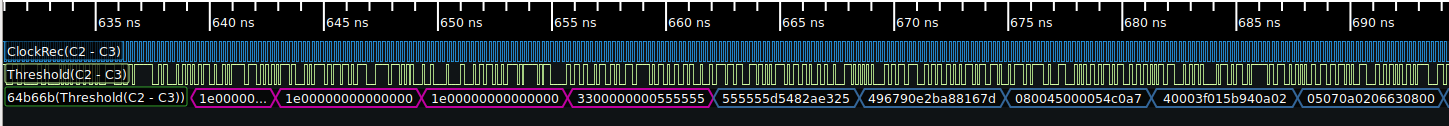
\includegraphics[width=16cm]{images/filters/64b66b.png}
\caption{Example 64b/66b decode}
\label{filter_64b66b}
\end{figure}

\subsection{Inputs}

\begin{tabularx}{16cm}{llX}
\thickhline
\textbf{Signal name} & \textbf{Type} & \textbf{Description} \\
\thickhline
data & 1-bit digital & Serial 8b/10b data line \\
\thickhline
clk & 1-bit digital & DDR bit clock, typically generated by use of the \hyperref[filter:cdrpll]{Clock Recovery
(PLL)} filter on the input data.\\
\thickhline
\end{tabularx}

\subsection{Parameters}

This filter takes no parameters.

\subsection{Output Signal}

The 64B/66B filter outputs a time series of 64B/66B sample objects. These consist of a control/data flag and
a 64-bit data block.

\begin{tabularx}{16cm}{lllX}
\thickhline
\textbf{Type} & \textbf{Description} & \textbf{Color} & \textbf{Format} \\
\thickhline
Control & Block with type 2'b10 & \cellcolor{control}\textcolor{white}{Control} & \%016x \\
\thickhline
Data & Block with type 2'b01 & \cellcolor{data}\textcolor{white}{Data} & \%016x \\
\thickhline
Error & Block with type 2'b00 or 2'b11 & \cellcolor{error}\textcolor{white}{Error} & \%016x \\
\thickhline
\end{tabularx}

%%%%%%%%%%%%%%%%%%%%%%%%%%%%%%%%%%%%%%%%%%%%%%%%%%%%%%%%%%%%%%%%%%%%%%%%%%%%%%%%%%%%%%%%%%%%%%%%%%%%%%%%%%%%%%%%%%%%%%%%
\pagebreak
\section{8B/10B (IBM)}
\label{filter:8b10b}

Decodes the standard 8b/10b line code used by SGMII, \hyperref[filter:1000basex]{1000base-X}, DisplayPort, JESD204,
\hyperref[filter:pcie2_logical]{PCIe gen 1/2}, SATA, USB 3.0, and many other common serial protocols.

8b/10b is a dictionary based code which converts each byte of message data to a ten-bit code. In order to maintain DC
balance and limit run length to a maximum of five identical bits in a row, all legal codes have one of:
\begin{itemize}
\item One legal coding, with exactly five zero bits
\item Two legal codings, one with four zero bits and one with six
\end{itemize}

The transmitter maintains a ``running disparity" counter and chooses the appropriate coding for each symbol to ensure
DC balance. There are twelve legal codes which are not needed for encoding data values; these are used to encode
frame boundaries, idle/alignment sequences, and other control information.

\begin{figure}[h]
\centering
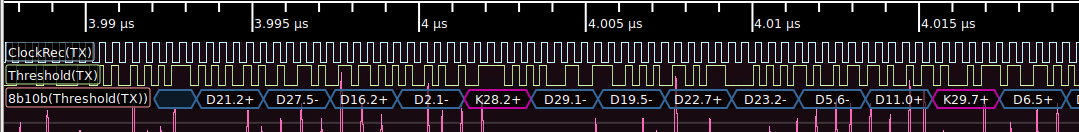
\includegraphics[width=16cm]{images/filters/8b10b.png}
\caption{Example 8b/10b decode}
\label{filter_8b10b}
\end{figure}

\subsection{Inputs}

\begin{tabularx}{16cm}{llX}
\thickhline
\textbf{Signal name} & \textbf{Type} & \textbf{Description} \\
\thickhline
data & 1-bit digital & Serial 8b/10b data line \\
\thickhline
clk & 1-bit digital & DDR bit clock, typically generated by use of the \hyperref[filter:cdrpll]{Clock Recovery
(PLL)} filter on the input data.\\
\thickhline
\end{tabularx}

\subsection{Parameters}

\begin{tabularx}{16cm}{llX}
\thickhline
\textbf{Parameter name} & \textbf{Type} & \textbf{Description} \\
\thickhline
Display Format & Enum &
	\textbf{Dotted (K28.5 D21.5)}: displays the 3b4b and 5b6b code blocks separately, with K or D prefix. \newline
	\textbf{Hex (K.bc b5)}: displays data as hex byte values and control codes with a K prefix. \\
\thickhline
\end{tabularx}

\subsection{Output Signal}

The 8B/10B filter outputs a time series of 8B/10B sample objects. These consist of a control/data flag and a byte of
data.

\begin{tabularx}{16cm}{lllX}
\thickhline
\textbf{Type} & \textbf{Description} & \textbf{Color} & \textbf{Format} \\
\thickhline
Control & Control codes & \cellcolor{control}\textcolor{white}{Control} & K\%d.\%d+ \\
\thickhline
Data & Upper layer protocol data & \cellcolor{data}\textcolor{white}{Data} & D\%d.\%d+ \\
\thickhline
Error & Malformed data & \cellcolor{error}\textcolor{white}{Error} & ERROR \\
\thickhline
\end{tabularx}

%%%%%%%%%%%%%%%%%%%%%%%%%%%%%%%%%%%%%%%%%%%%%%%%%%%%%%%%%%%%%%%%%%%%%%%%%%%%%%%%%%%%%%%%%%%%%%%%%%%%%%%%%%%%%%%%%%%%%%%%
\pagebreak
\section{8B/10B (TMDS)}
\label{filter:tmds}

Decodes the 8-to-10 Transition Minimized Differential Signalling line code used in \hyperref[filter:dvi]{DVI} and HDMI.

Like the \hyperref[filter:8b10b]{8B/10B (IBM)} line code, TMDS is an 8-to-10 bit serial line code. TMDS, however, is
designed to \emph{minimize} the number of toggles in the data stream for EMC reasons, rendering it difficult to
synchronize a CDR PLL to. As a result, HDMI and DVI provide a reference clock at the pixel clock rate (1/10 the serial
data bit rate) along with the data stream to provide synchronization.

\begin{figure}[h]
\centering
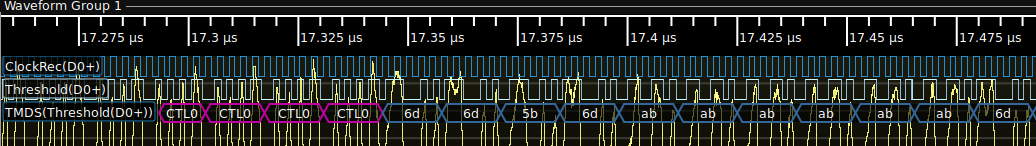
\includegraphics[width=16cm]{images/filters/tmds.png}
\caption{Example TMDS decode}
\label{filter_tmds}
\end{figure}

\subsection{Inputs}

\begin{tabularx}{16cm}{llX}
\thickhline
\textbf{Signal name} & \textbf{Type} & \textbf{Description} \\
\thickhline
data & 1-bit digital & Serial TMDS data line \\
\thickhline
clk & 1-bit digital & DDR \emph{bit} clock, typically generated by use of the \hyperref[filter:cdrpll]{Clock Recovery
(PLL)} filter on the input data. Note that this is 5x the rate of the pixel clock signal. \\
\thickhline
\end{tabularx}

\subsection{Parameters}

\begin{tabularx}{16cm}{llX}
\thickhline
\textbf{Parameter name} & \textbf{Type} & \textbf{Description} \\
\thickhline
Lane Number & Integer & Lane number within the link (0-3)\\
\thickhline
\end{tabularx}

\subsection{Output Signal}

The TMDS filter outputs a time series of TMDS sample objects. These consist of a type field and a byte of data.

The output of the TMDS decode is commonly fed to the \hyperref[filter:dvi]{DVI} or \hyperref[filter:hdmi]{HDMI}
protocol decoders.

\begin{tabularx}{16cm}{lllX}
\thickhline
\textbf{Type} & \textbf{Description} & \textbf{Color} & \textbf{Format} \\
\thickhline
Control & Control codes (H/V sync) & \cellcolor{control}\textcolor{white}{Control} & CTL\%d \\
\thickhline
Data & Pixel/island data & \cellcolor{data}\textcolor{white}{Data} & \%02x \\
\thickhline
Error & Malformed data & \cellcolor{error}\textcolor{white}{Error} & ERROR \\
\thickhline
Guard band & HDMI data/video guard band & \cellcolor{preamble}\textcolor{white}{Preamble} & GB \\
\thickhline
\end{tabularx}

%%%%%%%%%%%%%%%%%%%%%%%%%%%%%%%%%%%%%%%%%%%%%%%%%%%%%%%%%%%%%%%%%%%%%%%%%%%%%%%%%%%%%%%%%%%%%%%%%%%%%%%%%%%%%%%%%%%%%%%%
\pagebreak
\section{AC Couple}
\label{filter:accouple}

Automatically removes a DC offset from an analog waveform by subtracting the average of all samples from each sample.

This filter should only be used in postprocessing already acquired data, or other situations in which AC coupling in
the hardware (via an AC coupled probe, or coaxial DC block) is not possible.

\begin{figure}[h]
\centering
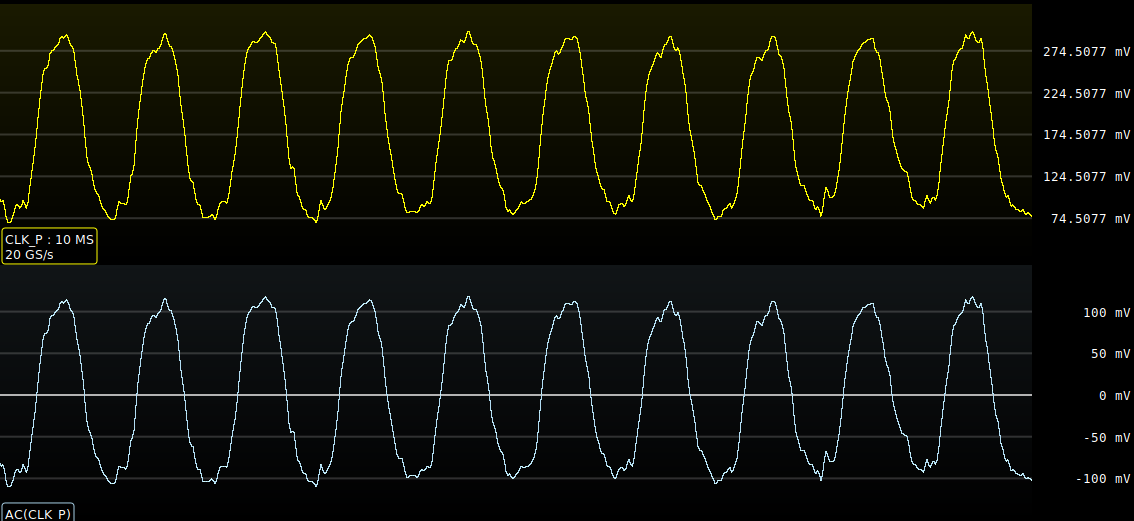
\includegraphics[width=16cm]{images/filters/ac-couple.png}
\caption{Example AC coupling}
\end{figure}

\subsection{Inputs}

\begin{tabularx}{16cm}{llX}
\thickhline
\textbf{Signal name} & \textbf{Type} & \textbf{Description} \\
\thickhline
din & Analog & Input waveform \\
\thickhline
\end{tabularx}

\subsection{Parameters}

This filter takes no parameters.

\subsection{Output Signal}

This filter outputs an analog waveform with identical sample rate to the input, vertically shifted to center the signal
at zero volts.

%%%%%%%%%%%%%%%%%%%%%%%%%%%%%%%%%%%%%%%%%%%%%%%%%%%%%%%%%%%%%%%%%%%%%%%%%%%%%%%%%%%%%%%%%%%%%%%%%%%%%%%%%%%%%%%%%%%%%%%%
\pagebreak
\section{ADL5205}
\label{filter:adl5205}

Decodes SPI data traffic to one half of an ADL5205 variable gain amplifier.

TODO: Screenshot

\subsection{Inputs}

\begin{tabularx}{16cm}{llX}
\thickhline
\textbf{Signal name} & \textbf{Type} & \textbf{Description} \\
\thickhline
spi & SPI bus & The SPI data bus \\
\thickhline
\end{tabularx}

\subsection{Parameters}

This filter takes no parameters.

\subsection{Output Signal}

This filter outputs one ADL5205 sample object for each write transaction, formatted as ``write: FA=2 dB, gain=8 dB".

%%%%%%%%%%%%%%%%%%%%%%%%%%%%%%%%%%%%%%%%%%%%%%%%%%%%%%%%%%%%%%%%%%%%%%%%%%%%%%%%%%%%%%%%%%%%%%%%%%%%%%%%%%%%%%%%%%%%%%%%
\pagebreak
\section{Autocorrelation}
\label{filter:autocorrelation}

This filter calculates the autocorrelation of an analog waveform. Autocorrelation is a measure of self-similarity
calculated by multiplying the signal with a time-shifted copy of itself. In Fig. \ref{filter_accouple}, strong peaks
can be seen at multiples of the 8b/10b symbol rate.

For best performance, it is crucial to keep the maximum offset as low as possible, since filter run time grows linearly
with offset range.

\begin{figure}[h]
\centering
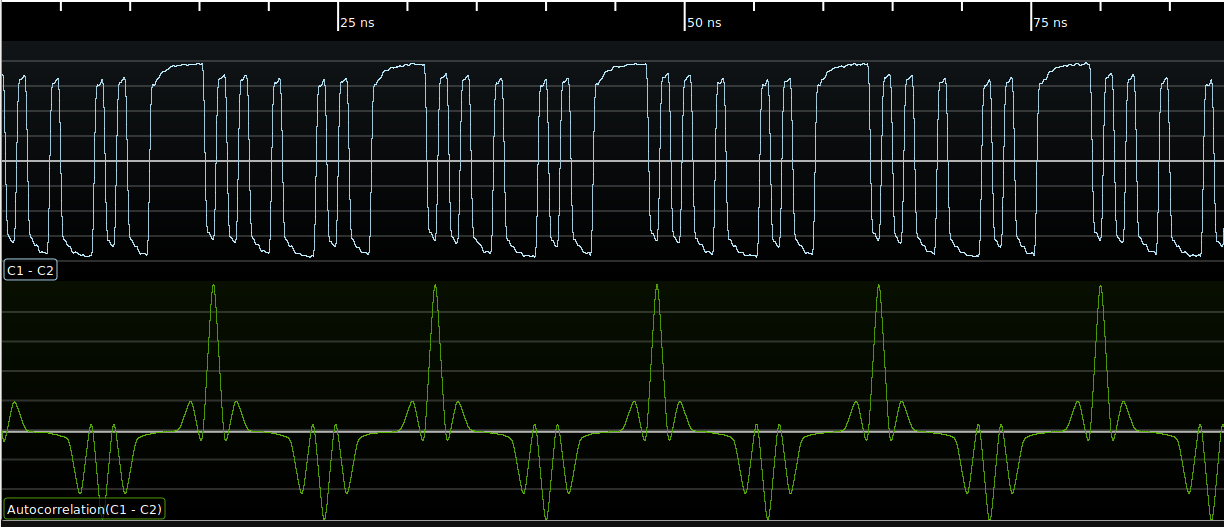
\includegraphics[width=16cm]{images/filters/autocorrelation.png}
\caption{Example of autocorrelation on a serial data stream}
\label{filter_accouple}
\end{figure}

\subsection{Inputs}

\begin{tabularx}{16cm}{llX}
\thickhline
\textbf{Signal name} & \textbf{Type} & \textbf{Description} \\
\thickhline
din & Analog & Input waveform \\
\thickhline
\end{tabularx}

\subsection{Parameters}

\begin{tabularx}{16cm}{llX}
\thickhline
\textbf{Parameter name} & \textbf{Type} & \textbf{Description} \\
\thickhline
Max offset & Integer & Maximum shift (in samples)\\
\thickhline
\end{tabularx}

\subsection{Output Signal}

This filter outputs an analog waveform with the same timebase as the input, one sample for each correlation offset.

%%%%%%%%%%%%%%%%%%%%%%%%%%%%%%%%%%%%%%%%%%%%%%%%%%%%%%%%%%%%%%%%%%%%%%%%%%%%%%%%%%%%%%%%%%%%%%%%%%%%%%%%%%%%%%%%%%%%%%%%
\pagebreak
\section{Base}
\label{filter:base}

Calculates the base (logical zero level) of each cycle in a digital waveform.

It is most commonly used as an input to statistics, to view the average base of the entire waveform. At times, however,
it may be useful to view the base waveform. For example, in Fig. \ref{filter_base}, the vertical eye closure caused by
channel ISI is readily apparent.

\begin{figure}[h]
\centering
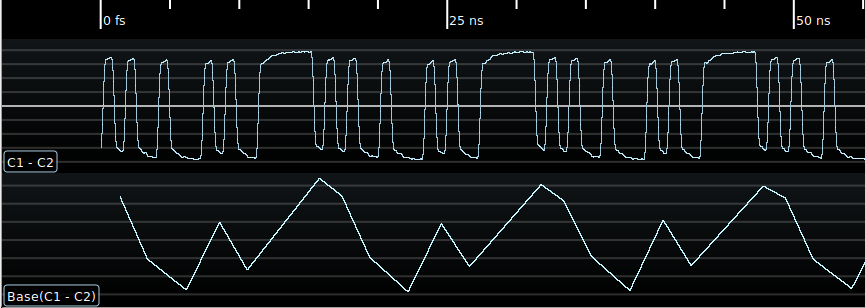
\includegraphics[width=16cm]{images/filters/base.png}
\caption{Example of base measurement on a serial data stream}
\label{filter_base}
\end{figure}

\subsection{Inputs}

\begin{tabularx}{16cm}{llX}
\thickhline
\textbf{Signal name} & \textbf{Type} & \textbf{Description} \\
\thickhline
din & Analog & Input waveform \\
\thickhline
\end{tabularx}

\subsection{Parameters}

This filter takes no parameters.

\subsection{Output Signal}

This filter outputs an analog waveform with one sample for each group of logical zeroes in the input signal, containing
the average value of the zero level for the middle 50\% of the low period.

%%%%%%%%%%%%%%%%%%%%%%%%%%%%%%%%%%%%%%%%%%%%%%%%%%%%%%%%%%%%%%%%%%%%%%%%%%%%%%%%%%%%%%%%%%%%%%%%%%%%%%%%%%%%%%%%%%%%%%%%
\pagebreak
\section{CAN}
\label{filter:can}

Decodes the Control Area Network (CAN) bus, commonly used in vehicle control systems. Both standard (11 bit) and
extended (29 bit) IDs are supported.

CAN-FD frames are detected and flagged as such, but the current decode cannot parse them fully.

\begin{figure}[h]
\centering
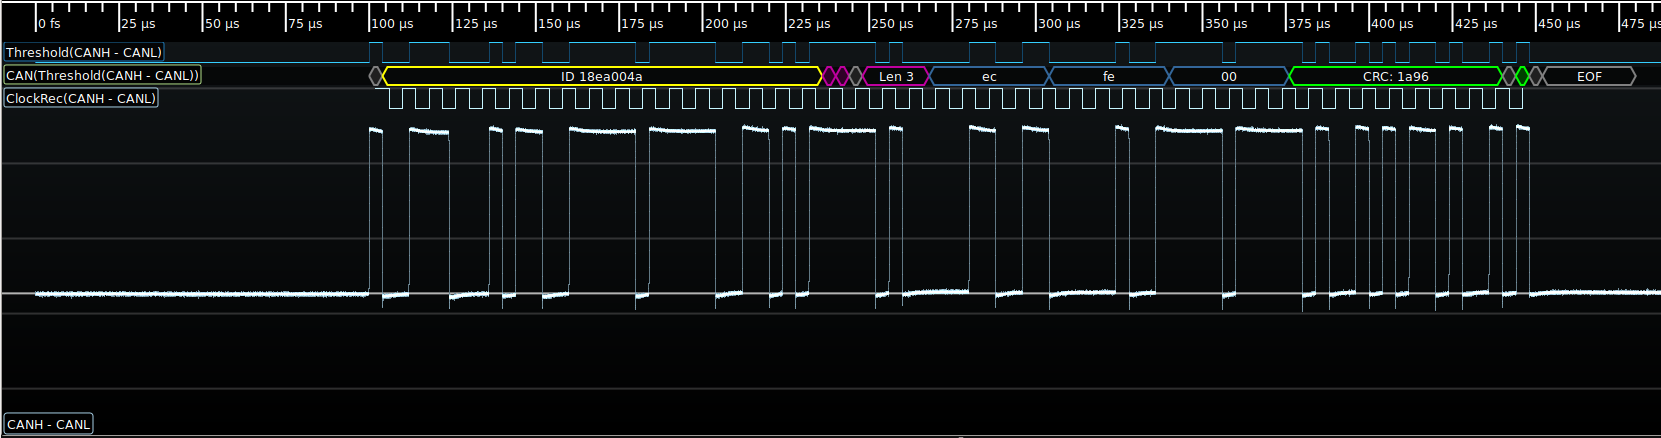
\includegraphics[width=16cm]{images/filters/can.png}
\caption{Example of CAN bus protocol decode}
\label{filter_can}
\end{figure}

\subsection{Inputs}

\begin{tabularx}{16cm}{llX}
\thickhline
\textbf{Signal name} & \textbf{Type} & \textbf{Description} \\
\thickhline
CANH & Digital & Thresholded CANH (or CANH-CANL) signal \\
\thickhline
\end{tabularx}

\subsection{Parameters}

\begin{tabularx}{16cm}{llX}
\thickhline
\textbf{Parameter name} & \textbf{Type} & \textbf{Description} \\
\thickhline
Bit Rate & Integer & Bit rate of the bus (most commonly 250 or 500 Kbps)\\
\thickhline
\end{tabularx}

\subsection{Output Signal}

The CAN bus decode outputs a time series of CAN sample objects. These consist of a type field and a byte of data.

\begin{tabularx}{16cm}{lllX}
\thickhline
\textbf{Type} & \textbf{Description} & \textbf{Color} & \textbf{Format} \\
\thickhline
Control & Start of frame & \cellcolor{preamble}\textcolor{white}{Preamble} & SOF \\
\thickhline
ID & CAN ID & \cellcolor{address}\textcolor{black}{Address} & ID \%x \\
\thickhline
RTR & Remote Transmission Request & \cellcolor{control}\textcolor{white}{Control} & DATA | REQ \\
\thickhline
FD mode & CAN-FD mode & \cellcolor{control}\textcolor{white}{Control} & FD | STD\\
\thickhline
R0 & Reserved bits & \cellcolor{preamble}\textcolor{white}{Preamble} & RSVD \\
\thickhline
DLC & Data Length Code & \cellcolor{control}\textcolor{white}{Control} & Len 3 \\
\thickhline
Data & Payload data & \cellcolor{data}\textcolor{white}{Data} & \%02x \\
\thickhline
Valid CRC & Good checksum & \cellcolor{checksumok}\textcolor{black}{Checksum OK} & CRC: \%04x \\
\thickhline
Invalid CRC & Bad checksum & \cellcolor{checksumbad}\textcolor{white}{Checksum Bad} & CRC: \%04x \\
\thickhline
CRC delimiter & Bus turnaround & \cellcolor{preamble}\textcolor{white}{Preamble} & CRC DELIM \\
\thickhline
ACK & Acknowledgement & \cellcolor{checksumok}\textcolor{black}{Checksum OK} & ACK \\
\thickhline
NAK & Missing acknowledgement & \cellcolor{checksumbad}\textcolor{white}{Checksum Bad} & NAK \\
\thickhline
ACK delimiter & Bus turnaround & \cellcolor{preamble}\textcolor{white}{Preamble} & ACK DELIM \\
\thickhline
EOF & End of frame & \cellcolor{preamble}\textcolor{white}{Preamble} & EOF \\

\thickhline
\end{tabularx}

%%%%%%%%%%%%%%%%%%%%%%%%%%%%%%%%%%%%%%%%%%%%%%%%%%%%%%%%%%%%%%%%%%%%%%%%%%%%%%%%%%%%%%%%%%%%%%%%%%%%%%%%%%%%%%%%%%%%%%%%
\pagebreak
\section{Channel Emulation}
\label{filter:channelemu}

This filter models the effects of applying an arbitrary channel, described via one or more 2-port S-parameter files, to
a waveform. Fig. \ref{filter_channelemu} shows the result of passing a 1.25 Gbps serial data pattern through a 10x
oscilloscope probe with approximately 500 MHz bandwidth. The ISI, attenuation, and phase shift introduced by the
channel can all be seen.

Only the forward path (S21) is considered in the current implementation of this filter; it is assumed that any
reflected power is absorbed by terminations at the transmitter. Channels with significant return loss reflecting off
the transmitter may not be modeled accurately.

The channel model works in the frequency domain. An FFT is performed on the input, then each complex point is
scaled by the interpolated S21 magnitude and rotated by the S21 phase, then an inverse FFT is used to transform the
signal back into the time domain. The group delay of the channel is estimated and samples are discarded from the
beginning of the waveform to prevent causality violations.

\begin{figure}[h]
\centering
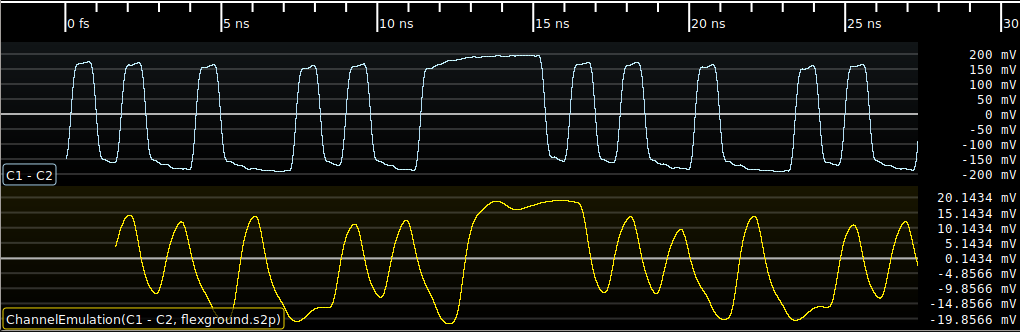
\includegraphics[width=16cm]{images/filters/channel-emulation.png}
\caption{Example of channel emulation on a serial data stream}
\label{filter_channelemu}
\end{figure}

\subsection{Inputs}

\begin{tabularx}{16cm}{llX}
\thickhline
\textbf{Signal name} & \textbf{Type} & \textbf{Description} \\
\thickhline
din & Analog & Input waveform \\
\thickhline
\end{tabularx}

\subsection{Parameters}

\begin{tabularx}{16cm}{llX}
\thickhline
\textbf{Parameter name} & \textbf{Type} & \textbf{Description} \\
\thickhline
S-Parameters & Filename vector & List of S-parameter files describing the channel\\
\thickhline
\end{tabularx}

\subsection{Output Signal}

This filter outputs an analog waveform with the same timebase as the input, with the emulated channel applied.

%%%%%%%%%%%%%%%%%%%%%%%%%%%%%%%%%%%%%%%%%%%%%%%%%%%%%%%%%%%%%%%%%%%%%%%%%%%%%%%%%%%%%%%%%%%%%%%%%%%%%%%%%%%%%%%%%%%%%%%%
\pagebreak
\section{Clock Recovery (D-PHY HS Mode)}

Extracts a double-rate clock from a MIPI D-PHY clock+data stream, which is gated to only toggle when the data input
is in HS mode. This can be used for generating eye patterns of the HS-mode data.

%%%%%%%%%%%%%%%%%%%%%%%%%%%%%%%%%%%%%%%%%%%%%%%%%%%%%%%%%%%%%%%%%%%%%%%%%%%%%%%%%%%%%%%%%%%%%%%%%%%%%%%%%%%%%%%%%%%%%%%%
\pagebreak
\section{Clock Recovery (PLL)}
\label{filter:cdrpll}

%%%%%%%%%%%%%%%%%%%%%%%%%%%%%%%%%%%%%%%%%%%%%%%%%%%%%%%%%%%%%%%%%%%%%%%%%%%%%%%%%%%%%%%%%%%%%%%%%%%%%%%%%%%%%%%%%%%%%%%%
\pagebreak
\section{Clock Recovery (UART)}

%%%%%%%%%%%%%%%%%%%%%%%%%%%%%%%%%%%%%%%%%%%%%%%%%%%%%%%%%%%%%%%%%%%%%%%%%%%%%%%%%%%%%%%%%%%%%%%%%%%%%%%%%%%%%%%%%%%%%%%%
\pagebreak
\section{Current Shunt}

Converts a voltage waveform acquired across a known resistance into a current waveform.

%%%%%%%%%%%%%%%%%%%%%%%%%%%%%%%%%%%%%%%%%%%%%%%%%%%%%%%%%%%%%%%%%%%%%%%%%%%%%%%%%%%%%%%%%%%%%%%%%%%%%%%%%%%%%%%%%%%%%%%%
\pagebreak
\section{DC Offset}

Adds a constant value to each sample in an analog waveform.

\subsection{Inputs}

\begin{tabularx}{16cm}{llX}
\thickhline
\textbf{Signal name} & \textbf{Type} & \textbf{Description} \\
\thickhline
din & Analog & Input waveform \\
\thickhline
\end{tabularx}

\subsection{Parameters}

\begin{tabularx}{16cm}{llX}
\thickhline
\textbf{Parameter name} & \textbf{Type} & \textbf{Description} \\
\thickhline
Offset & Float & The offset to apply \\
\thickhline
\end{tabularx}

\subsection{Output Signal}

This filter outputs an analog waveform with one sample for each sample in the input, shifted by the requested offset.

%%%%%%%%%%%%%%%%%%%%%%%%%%%%%%%%%%%%%%%%%%%%%%%%%%%%%%%%%%%%%%%%%%%%%%%%%%%%%%%%%%%%%%%%%%%%%%%%%%%%%%%%%%%%%%%%%%%%%%%%
\pagebreak
\section{DDJ}

Calculates data-dependent jitter for a serial data stream.

%%%%%%%%%%%%%%%%%%%%%%%%%%%%%%%%%%%%%%%%%%%%%%%%%%%%%%%%%%%%%%%%%%%%%%%%%%%%%%%%%%%%%%%%%%%%%%%%%%%%%%%%%%%%%%%%%%%%%%%%
\pagebreak
\section{DDR1 Command Bus}

Decodes the command bus for first-generation DDR SDRAM.

%%%%%%%%%%%%%%%%%%%%%%%%%%%%%%%%%%%%%%%%%%%%%%%%%%%%%%%%%%%%%%%%%%%%%%%%%%%%%%%%%%%%%%%%%%%%%%%%%%%%%%%%%%%%%%%%%%%%%%%%
\pagebreak
\section{DDR3 Command Bus}

Decodes the command bus for third-generation DDR SDRAM.

%%%%%%%%%%%%%%%%%%%%%%%%%%%%%%%%%%%%%%%%%%%%%%%%%%%%%%%%%%%%%%%%%%%%%%%%%%%%%%%%%%%%%%%%%%%%%%%%%%%%%%%%%%%%%%%%%%%%%%%%
\pagebreak
\section{De-Embed}

Applies the inverse of a channel (supplied in 2-port Touchstone S-parameter format) to a signal, in order to calculate
what the waveform would have looked like at the input to a cable, fixture, etc. given the signal seen at the output.

Multiple Touchstone files may be provided, however only transmission (S21) is modeled in the current implementation so
cascading channels or filters which have significant return loss may lead to inaccurate results (signals reflecting
between two elements then back in the forward direction are not modeled).

%%%%%%%%%%%%%%%%%%%%%%%%%%%%%%%%%%%%%%%%%%%%%%%%%%%%%%%%%%%%%%%%%%%%%%%%%%%%%%%%%%%%%%%%%%%%%%%%%%%%%%%%%%%%%%%%%%%%%%%%
\pagebreak
\section{Deskew}

Moves an analog waveform earlier or later in time to compensate for trigger offsets, probe length mismatch, etc.
It is generally preferable to deskew using the skew adjustment on the channel during acquisition; this filter is
provided for correction in postprocessing.

\subsection{Inputs}

\begin{tabularx}{16cm}{llX}
\thickhline
\textbf{Signal name} & \textbf{Type} & \textbf{Description} \\
\thickhline
din & Analog & Input waveform \\
\thickhline
\end{tabularx}

\subsection{Parameters}

\begin{tabularx}{16cm}{llX}
\thickhline
\textbf{Parameter name} & \textbf{Type} & \textbf{Description} \\
\thickhline
Skew & Float & Time offset to shift the waveform\\
\thickhline
\end{tabularx}

\subsection{Output Signal}

This filter outputs an analog waveform with one sample for each sample in the input, phase shifted by the requested
offset.

%%%%%%%%%%%%%%%%%%%%%%%%%%%%%%%%%%%%%%%%%%%%%%%%%%%%%%%%%%%%%%%%%%%%%%%%%%%%%%%%%%%%%%%%%%%%%%%%%%%%%%%%%%%%%%%%%%%%%%%%
\pagebreak
\section{Downconvert}

Performs digital downconversion by mixing a directly sampled RF signal with a two-phase local oscillator, then outputs
the downconverted signal. No filtering or decimation is performed.

%%%%%%%%%%%%%%%%%%%%%%%%%%%%%%%%%%%%%%%%%%%%%%%%%%%%%%%%%%%%%%%%%%%%%%%%%%%%%%%%%%%%%%%%%%%%%%%%%%%%%%%%%%%%%%%%%%%%%%%%
\pagebreak
\section{Downsample}

Low-pass filters a signal to prevent aliasing, then decimates by an integer factor.

%%%%%%%%%%%%%%%%%%%%%%%%%%%%%%%%%%%%%%%%%%%%%%%%%%%%%%%%%%%%%%%%%%%%%%%%%%%%%%%%%%%%%%%%%%%%%%%%%%%%%%%%%%%%%%%%%%%%%%%%
\pagebreak
\section{DRAM Clocks}

Given a DRAM command bus and a DQS strobe, produce separate gated DQ clock streams for read and write bursts.

%%%%%%%%%%%%%%%%%%%%%%%%%%%%%%%%%%%%%%%%%%%%%%%%%%%%%%%%%%%%%%%%%%%%%%%%%%%%%%%%%%%%%%%%%%%%%%%%%%%%%%%%%%%%%%%%%%%%%%%%
\pagebreak
\section{DRAM Trcd}

%%%%%%%%%%%%%%%%%%%%%%%%%%%%%%%%%%%%%%%%%%%%%%%%%%%%%%%%%%%%%%%%%%%%%%%%%%%%%%%%%%%%%%%%%%%%%%%%%%%%%%%%%%%%%%%%%%%%%%%%
\pagebreak
\section{DRAM Trfc}

%%%%%%%%%%%%%%%%%%%%%%%%%%%%%%%%%%%%%%%%%%%%%%%%%%%%%%%%%%%%%%%%%%%%%%%%%%%%%%%%%%%%%%%%%%%%%%%%%%%%%%%%%%%%%%%%%%%%%%%%
\pagebreak
\section{Duty Cycle}

Calculates the duty cycle of a bimodal waveform. The duty cycle is defined as the percentage of time spent in the high
state divided by the period.

%%%%%%%%%%%%%%%%%%%%%%%%%%%%%%%%%%%%%%%%%%%%%%%%%%%%%%%%%%%%%%%%%%%%%%%%%%%%%%%%%%%%%%%%%%%%%%%%%%%%%%%%%%%%%%%%%%%%%%%%
\pagebreak
\section{DVI}
\label{filter:dvi}

%%%%%%%%%%%%%%%%%%%%%%%%%%%%%%%%%%%%%%%%%%%%%%%%%%%%%%%%%%%%%%%%%%%%%%%%%%%%%%%%%%%%%%%%%%%%%%%%%%%%%%%%%%%%%%%%%%%%%%%%
\pagebreak
\section{Emphasis}

Adds pre/de emphasis to a signal.

%%%%%%%%%%%%%%%%%%%%%%%%%%%%%%%%%%%%%%%%%%%%%%%%%%%%%%%%%%%%%%%%%%%%%%%%%%%%%%%%%%%%%%%%%%%%%%%%%%%%%%%%%%%%%%%%%%%%%%%%
\pagebreak
\section{Emphasis Removal}

Removes pre/de emphasis from a signal.

%%%%%%%%%%%%%%%%%%%%%%%%%%%%%%%%%%%%%%%%%%%%%%%%%%%%%%%%%%%%%%%%%%%%%%%%%%%%%%%%%%%%%%%%%%%%%%%%%%%%%%%%%%%%%%%%%%%%%%%%
\pagebreak
\section{Ethernet - 10baseT}

%%%%%%%%%%%%%%%%%%%%%%%%%%%%%%%%%%%%%%%%%%%%%%%%%%%%%%%%%%%%%%%%%%%%%%%%%%%%%%%%%%%%%%%%%%%%%%%%%%%%%%%%%%%%%%%%%%%%%%%%
\pagebreak
\section{Ethernet - 100baseTX}

%%%%%%%%%%%%%%%%%%%%%%%%%%%%%%%%%%%%%%%%%%%%%%%%%%%%%%%%%%%%%%%%%%%%%%%%%%%%%%%%%%%%%%%%%%%%%%%%%%%%%%%%%%%%%%%%%%%%%%%%
\pagebreak
\section{Ethernet - 1000baseX}
\label{proto:1000basex}

Decodes the 1000base-X Ethernet PCS as specified in IEEE 802.3 clause 36.

\begin{tabularx}{16cm}{llX}
\thickhline
\textbf{Signal name} & \textbf{Type} & \textbf{Description} \\
\thickhline
data & 8b/10b & Output of \hyperref[proto:8b10b]{8b/10b protocol decode}\\
\thickhline
\end{tabularx}

\subsection{Parameters}

This filter takes no parameters.

\subsection{Output Signal}

The 1000base-X filter outputs a series of Ethernet frame segment objects.

\begin{tabularx}{16cm}{lllX}
\thickhline
\textbf{Type} & \textbf{Description} & \textbf{Color} & \textbf{Format} \\
\thickhline
Preamble & Preamble & \cellcolor{preamble}\textcolor{white}{Preamble} & PREAMBLE \\
\thickhline
Preamble & Start of frame delimiter & \cellcolor{preamble}\textcolor{white}{Preamble} & SFD \\
\thickhline
Address & Src/dest MAC & \cellcolor{address}\textcolor{black}{Address} & From 02:00:11:22:33:44 \\
\thickhline
Control & Ethertype & \cellcolor{control}\textcolor{white}{Control} & Type: IPv4 \newline Type: 0xbeef \\
\thickhline
Control & VLAN tag & \cellcolor{control}\textcolor{white}{Control} & VLAN 10, PCP 0 \\
\thickhline
Data & Frame data & \cellcolor{data}\textcolor{white}{Data} & a5 \\
\thickhline
Checksum OK & Valid FCS & \cellcolor{checksumok}\textcolor{black}{Checksum OK} & CRC: 0xdeadbeef \\
\thickhline
Checksum Bad & Invalid FCS & \cellcolor{checksumbad}\textcolor{white}{Checksum Bad} & CRC: 0xbaadc0de \\
\thickhline
Error & Malformed data & \cellcolor{error}\textcolor{white}{Error} & ERROR \\
\thickhline
\end{tabularx}

TODO: Document protocol analyzer output

%%%%%%%%%%%%%%%%%%%%%%%%%%%%%%%%%%%%%%%%%%%%%%%%%%%%%%%%%%%%%%%%%%%%%%%%%%%%%%%%%%%%%%%%%%%%%%%%%%%%%%%%%%%%%%%%%%%%%%%%
\pagebreak
\section{Ethernet - GMII}

%%%%%%%%%%%%%%%%%%%%%%%%%%%%%%%%%%%%%%%%%%%%%%%%%%%%%%%%%%%%%%%%%%%%%%%%%%%%%%%%%%%%%%%%%%%%%%%%%%%%%%%%%%%%%%%%%%%%%%%%
\pagebreak
\section{Ethernet - RGMII}

%%%%%%%%%%%%%%%%%%%%%%%%%%%%%%%%%%%%%%%%%%%%%%%%%%%%%%%%%%%%%%%%%%%%%%%%%%%%%%%%%%%%%%%%%%%%%%%%%%%%%%%%%%%%%%%%%%%%%%%%
\pagebreak
\section{Ethernet Autonegotiation}

%%%%%%%%%%%%%%%%%%%%%%%%%%%%%%%%%%%%%%%%%%%%%%%%%%%%%%%%%%%%%%%%%%%%%%%%%%%%%%%%%%%%%%%%%%%%%%%%%%%%%%%%%%%%%%%%%%%%%%%%
\pagebreak
\section{Eye Bit Rate}

%%%%%%%%%%%%%%%%%%%%%%%%%%%%%%%%%%%%%%%%%%%%%%%%%%%%%%%%%%%%%%%%%%%%%%%%%%%%%%%%%%%%%%%%%%%%%%%%%%%%%%%%%%%%%%%%%%%%%%%%
\pagebreak
\section{Eye Height}

%%%%%%%%%%%%%%%%%%%%%%%%%%%%%%%%%%%%%%%%%%%%%%%%%%%%%%%%%%%%%%%%%%%%%%%%%%%%%%%%%%%%%%%%%%%%%%%%%%%%%%%%%%%%%%%%%%%%%%%%
\pagebreak
\section{Eye P-P Jitter}

%%%%%%%%%%%%%%%%%%%%%%%%%%%%%%%%%%%%%%%%%%%%%%%%%%%%%%%%%%%%%%%%%%%%%%%%%%%%%%%%%%%%%%%%%%%%%%%%%%%%%%%%%%%%%%%%%%%%%%%%
\pagebreak
\section{Eye Pattern}

%%%%%%%%%%%%%%%%%%%%%%%%%%%%%%%%%%%%%%%%%%%%%%%%%%%%%%%%%%%%%%%%%%%%%%%%%%%%%%%%%%%%%%%%%%%%%%%%%%%%%%%%%%%%%%%%%%%%%%%%
\pagebreak
\section{Eye Period}

%%%%%%%%%%%%%%%%%%%%%%%%%%%%%%%%%%%%%%%%%%%%%%%%%%%%%%%%%%%%%%%%%%%%%%%%%%%%%%%%%%%%%%%%%%%%%%%%%%%%%%%%%%%%%%%%%%%%%%%%
\pagebreak
\section{Eye Width}

%%%%%%%%%%%%%%%%%%%%%%%%%%%%%%%%%%%%%%%%%%%%%%%%%%%%%%%%%%%%%%%%%%%%%%%%%%%%%%%%%%%%%%%%%%%%%%%%%%%%%%%%%%%%%%%%%%%%%%%%
\pagebreak
\section{Fall}

%%%%%%%%%%%%%%%%%%%%%%%%%%%%%%%%%%%%%%%%%%%%%%%%%%%%%%%%%%%%%%%%%%%%%%%%%%%%%%%%%%%%%%%%%%%%%%%%%%%%%%%%%%%%%%%%%%%%%%%%
\pagebreak
\section{FFT}

%%%%%%%%%%%%%%%%%%%%%%%%%%%%%%%%%%%%%%%%%%%%%%%%%%%%%%%%%%%%%%%%%%%%%%%%%%%%%%%%%%%%%%%%%%%%%%%%%%%%%%%%%%%%%%%%%%%%%%%%
\pagebreak
\section{FIR}

Applies a finite-impulse-response filter to a signal.

%%%%%%%%%%%%%%%%%%%%%%%%%%%%%%%%%%%%%%%%%%%%%%%%%%%%%%%%%%%%%%%%%%%%%%%%%%%%%%%%%%%%%%%%%%%%%%%%%%%%%%%%%%%%%%%%%%%%%%%%
\pagebreak
\section{Frequency}

%%%%%%%%%%%%%%%%%%%%%%%%%%%%%%%%%%%%%%%%%%%%%%%%%%%%%%%%%%%%%%%%%%%%%%%%%%%%%%%%%%%%%%%%%%%%%%%%%%%%%%%%%%%%%%%%%%%%%%%%
\pagebreak
\section{Horizontal Bathtub}

%%%%%%%%%%%%%%%%%%%%%%%%%%%%%%%%%%%%%%%%%%%%%%%%%%%%%%%%%%%%%%%%%%%%%%%%%%%%%%%%%%%%%%%%%%%%%%%%%%%%%%%%%%%%%%%%%%%%%%%%
\pagebreak
\section{HDMI}
\label{filter:hdmi}

%%%%%%%%%%%%%%%%%%%%%%%%%%%%%%%%%%%%%%%%%%%%%%%%%%%%%%%%%%%%%%%%%%%%%%%%%%%%%%%%%%%%%%%%%%%%%%%%%%%%%%%%%%%%%%%%%%%%%%%%
\pagebreak
\section{$I^2C$}

%%%%%%%%%%%%%%%%%%%%%%%%%%%%%%%%%%%%%%%%%%%%%%%%%%%%%%%%%%%%%%%%%%%%%%%%%%%%%%%%%%%%%%%%%%%%%%%%%%%%%%%%%%%%%%%%%%%%%%%%
\pagebreak
\section{$I^2C$ EEPROM}

Decodes common $I^2C$ EEPROM memory devices

%%%%%%%%%%%%%%%%%%%%%%%%%%%%%%%%%%%%%%%%%%%%%%%%%%%%%%%%%%%%%%%%%%%%%%%%%%%%%%%%%%%%%%%%%%%%%%%%%%%%%%%%%%%%%%%%%%%%%%%%
\pagebreak
\section{Intel eSPI}

Decodes the Enhanced Serial Peripheral Interface protocol, used between Intel CPUs and peripherals such as baseboard
management controllers (BMCs) and embedded controllers (ECs).

%%%%%%%%%%%%%%%%%%%%%%%%%%%%%%%%%%%%%%%%%%%%%%%%%%%%%%%%%%%%%%%%%%%%%%%%%%%%%%%%%%%%%%%%%%%%%%%%%%%%%%%%%%%%%%%%%%%%%%%%
\pagebreak
\section{IPv4}

%%%%%%%%%%%%%%%%%%%%%%%%%%%%%%%%%%%%%%%%%%%%%%%%%%%%%%%%%%%%%%%%%%%%%%%%%%%%%%%%%%%%%%%%%%%%%%%%%%%%%%%%%%%%%%%%%%%%%%%%
\pagebreak
\section{Jitter Spectrum}

%%%%%%%%%%%%%%%%%%%%%%%%%%%%%%%%%%%%%%%%%%%%%%%%%%%%%%%%%%%%%%%%%%%%%%%%%%%%%%%%%%%%%%%%%%%%%%%%%%%%%%%%%%%%%%%%%%%%%%%%
\pagebreak
\section{JTAG}

%%%%%%%%%%%%%%%%%%%%%%%%%%%%%%%%%%%%%%%%%%%%%%%%%%%%%%%%%%%%%%%%%%%%%%%%%%%%%%%%%%%%%%%%%%%%%%%%%%%%%%%%%%%%%%%%%%%%%%%%
\pagebreak
\section{Magnitude}

Calculates the magnitude of a complex valued signal

%%%%%%%%%%%%%%%%%%%%%%%%%%%%%%%%%%%%%%%%%%%%%%%%%%%%%%%%%%%%%%%%%%%%%%%%%%%%%%%%%%%%%%%%%%%%%%%%%%%%%%%%%%%%%%%%%%%%%%%%
\pagebreak
\section{MDIO}

Decodes the Management Data Input/Output interface on Ethernet PHYs. At the moment, only Clause 22 format is supported.

%%%%%%%%%%%%%%%%%%%%%%%%%%%%%%%%%%%%%%%%%%%%%%%%%%%%%%%%%%%%%%%%%%%%%%%%%%%%%%%%%%%%%%%%%%%%%%%%%%%%%%%%%%%%%%%%%%%%%%%%
\pagebreak
\section{MIL-STD-1553}

Decodes the MIL-STD-1553 avionics data bus.

%%%%%%%%%%%%%%%%%%%%%%%%%%%%%%%%%%%%%%%%%%%%%%%%%%%%%%%%%%%%%%%%%%%%%%%%%%%%%%%%%%%%%%%%%%%%%%%%%%%%%%%%%%%%%%%%%%%%%%%%
\pagebreak
\section{MIPI D-Phy Data}

Converts two streams of D-Phy Symbol's (one data and one clock) into bytes and control events

%%%%%%%%%%%%%%%%%%%%%%%%%%%%%%%%%%%%%%%%%%%%%%%%%%%%%%%%%%%%%%%%%%%%%%%%%%%%%%%%%%%%%%%%%%%%%%%%%%%%%%%%%%%%%%%%%%%%%%%%
\pagebreak
\section{MIPI D-Phy Symbol}

Decodes one or two analog channels to MIPI D-PHY symbols (HS/LS line states). Either the positive half, or both
positive and negative, of the pair may be provided.

If only the positive half is provided, it is possible to decode HS data and clocks, but not the LP-01 and LP-10 states,
as these are indistinguishable from LP-00 and LP-11. This prevents proper decoding of Escape Mode data, although
Start-Of-Transmission sequences may be inferred from context.

%%%%%%%%%%%%%%%%%%%%%%%%%%%%%%%%%%%%%%%%%%%%%%%%%%%%%%%%%%%%%%%%%%%%%%%%%%%%%%%%%%%%%%%%%%%%%%%%%%%%%%%%%%%%%%%%%%%%%%%%
\pagebreak
\section{MIPI DSI Frame}

Converts a MIPI DSI Packet stream into video scanlines.

%%%%%%%%%%%%%%%%%%%%%%%%%%%%%%%%%%%%%%%%%%%%%%%%%%%%%%%%%%%%%%%%%%%%%%%%%%%%%%%%%%%%%%%%%%%%%%%%%%%%%%%%%%%%%%%%%%%%%%%%
\pagebreak
\section{MIPI DSI Packet}

Converts two streams of D-Phy Symbol's (one data and one clock) into MIPI DSI packets.

%%%%%%%%%%%%%%%%%%%%%%%%%%%%%%%%%%%%%%%%%%%%%%%%%%%%%%%%%%%%%%%%%%%%%%%%%%%%%%%%%%%%%%%%%%%%%%%%%%%%%%%%%%%%%%%%%%%%%%%%
\pagebreak
\section{Moving Average}

%%%%%%%%%%%%%%%%%%%%%%%%%%%%%%%%%%%%%%%%%%%%%%%%%%%%%%%%%%%%%%%%%%%%%%%%%%%%%%%%%%%%%%%%%%%%%%%%%%%%%%%%%%%%%%%%%%%%%%%%
\pagebreak
\section{Multiply}

Multiplies one waveform by another. No resampling is performed; both inputs must have identical sample rates.

Unit conversions are performed, for example the product of a voltage and current waveform is a power waveform.

%%%%%%%%%%%%%%%%%%%%%%%%%%%%%%%%%%%%%%%%%%%%%%%%%%%%%%%%%%%%%%%%%%%%%%%%%%%%%%%%%%%%%%%%%%%%%%%%%%%%%%%%%%%%%%%%%%%%%%%%
\pagebreak
\section{OFDM Demodulator}

NOTE: this filter is still under development and not suitable for general use.

%%%%%%%%%%%%%%%%%%%%%%%%%%%%%%%%%%%%%%%%%%%%%%%%%%%%%%%%%%%%%%%%%%%%%%%%%%%%%%%%%%%%%%%%%%%%%%%%%%%%%%%%%%%%%%%%%%%%%%%%
\pagebreak
\section{Overshoot}

%%%%%%%%%%%%%%%%%%%%%%%%%%%%%%%%%%%%%%%%%%%%%%%%%%%%%%%%%%%%%%%%%%%%%%%%%%%%%%%%%%%%%%%%%%%%%%%%%%%%%%%%%%%%%%%%%%%%%%%%
\pagebreak
\section{Parallel Bus}

%%%%%%%%%%%%%%%%%%%%%%%%%%%%%%%%%%%%%%%%%%%%%%%%%%%%%%%%%%%%%%%%%%%%%%%%%%%%%%%%%%%%%%%%%%%%%%%%%%%%%%%%%%%%%%%%%%%%%%%%
\pagebreak
\section{PCIe Data Link}

Decodes the Data Link layer of PCI Express. At this layer DLLPs are fully decoded. TLP sequence numbers are visible
and CRC16s are checked, however TLP content is displayed as hex dumps.

%%%%%%%%%%%%%%%%%%%%%%%%%%%%%%%%%%%%%%%%%%%%%%%%%%%%%%%%%%%%%%%%%%%%%%%%%%%%%%%%%%%%%%%%%%%%%%%%%%%%%%%%%%%%%%%%%%%%%%%%
\pagebreak
\section{PCIe Gen 1/2 Logical}

Decodes the Logical Sub-Block of the PCI Express 1.0 and 2.0 PHY. This layer decodes 8B/10B symbols and the LFSR
scrambler. TLP and DLLP start/end markers are identified but no packet decoding is performed.

%%%%%%%%%%%%%%%%%%%%%%%%%%%%%%%%%%%%%%%%%%%%%%%%%%%%%%%%%%%%%%%%%%%%%%%%%%%%%%%%%%%%%%%%%%%%%%%%%%%%%%%%%%%%%%%%%%%%%%%%
\pagebreak
\section{PCIe Transport}

Decodes the Transport layer of PCI Express. At this layer TLPs are fully decoded, however only a unidirectional view
of the system is visible (only TX or only RX).

%%%%%%%%%%%%%%%%%%%%%%%%%%%%%%%%%%%%%%%%%%%%%%%%%%%%%%%%%%%%%%%%%%%%%%%%%%%%%%%%%%%%%%%%%%%%%%%%%%%%%%%%%%%%%%%%%%%%%%%%
\pagebreak
\section{Peak Hold}

%%%%%%%%%%%%%%%%%%%%%%%%%%%%%%%%%%%%%%%%%%%%%%%%%%%%%%%%%%%%%%%%%%%%%%%%%%%%%%%%%%%%%%%%%%%%%%%%%%%%%%%%%%%%%%%%%%%%%%%%
\pagebreak
\section{Peak-to-Peak}

%%%%%%%%%%%%%%%%%%%%%%%%%%%%%%%%%%%%%%%%%%%%%%%%%%%%%%%%%%%%%%%%%%%%%%%%%%%%%%%%%%%%%%%%%%%%%%%%%%%%%%%%%%%%%%%%%%%%%%%%
\pagebreak
\section{Period}

%%%%%%%%%%%%%%%%%%%%%%%%%%%%%%%%%%%%%%%%%%%%%%%%%%%%%%%%%%%%%%%%%%%%%%%%%%%%%%%%%%%%%%%%%%%%%%%%%%%%%%%%%%%%%%%%%%%%%%%%
\pagebreak
\section{Rj + BUj}

Removes data-dependent jitter (DDJ) from a TIE waveform, leaving uncorrelated jitter (Rj and BUj).

%%%%%%%%%%%%%%%%%%%%%%%%%%%%%%%%%%%%%%%%%%%%%%%%%%%%%%%%%%%%%%%%%%%%%%%%%%%%%%%%%%%%%%%%%%%%%%%%%%%%%%%%%%%%%%%%%%%%%%%%
\pagebreak
\section{QSPI}

Quad SPI as used in serial Flash. Note that this filter \emph{only} decodes quad mode streams, not x1 SPI.

%%%%%%%%%%%%%%%%%%%%%%%%%%%%%%%%%%%%%%%%%%%%%%%%%%%%%%%%%%%%%%%%%%%%%%%%%%%%%%%%%%%%%%%%%%%%%%%%%%%%%%%%%%%%%%%%%%%%%%%%
\pagebreak
\section{Quadrature}

Quadrature pulses from a rotary encoder

%%%%%%%%%%%%%%%%%%%%%%%%%%%%%%%%%%%%%%%%%%%%%%%%%%%%%%%%%%%%%%%%%%%%%%%%%%%%%%%%%%%%%%%%%%%%%%%%%%%%%%%%%%%%%%%%%%%%%%%%
\pagebreak
\section{Rise}

Calculates the rise time for each cycle of a waveform

%%%%%%%%%%%%%%%%%%%%%%%%%%%%%%%%%%%%%%%%%%%%%%%%%%%%%%%%%%%%%%%%%%%%%%%%%%%%%%%%%%%%%%%%%%%%%%%%%%%%%%%%%%%%%%%%%%%%%%%%
\pagebreak
\section{SD Card Command}

Decodes the Secure Digital card command bus protocol

%%%%%%%%%%%%%%%%%%%%%%%%%%%%%%%%%%%%%%%%%%%%%%%%%%%%%%%%%%%%%%%%%%%%%%%%%%%%%%%%%%%%%%%%%%%%%%%%%%%%%%%%%%%%%%%%%%%%%%%%
\pagebreak
\section{Spectrogram}

Displays a 2D plot of frequency vs time using configurable FFT length.

%%%%%%%%%%%%%%%%%%%%%%%%%%%%%%%%%%%%%%%%%%%%%%%%%%%%%%%%%%%%%%%%%%%%%%%%%%%%%%%%%%%%%%%%%%%%%%%%%%%%%%%%%%%%%%%%%%%%%%%%
\pagebreak
\section{SPI}

Serial Peripheral Interface.

%%%%%%%%%%%%%%%%%%%%%%%%%%%%%%%%%%%%%%%%%%%%%%%%%%%%%%%%%%%%%%%%%%%%%%%%%%%%%%%%%%%%%%%%%%%%%%%%%%%%%%%%%%%%%%%%%%%%%%%%
\pagebreak
\section{SPI Flash}

Flash memory attached to a SPI or quad SPI bus. Typically these chips have part numbers that start with ``25".

%%%%%%%%%%%%%%%%%%%%%%%%%%%%%%%%%%%%%%%%%%%%%%%%%%%%%%%%%%%%%%%%%%%%%%%%%%%%%%%%%%%%%%%%%%%%%%%%%%%%%%%%%%%%%%%%%%%%%%%%
\pagebreak
\section{Subtract}


Subtracts one waveform from another. No resampling is performed; both inputs must have identical sample rates.

\subsection{Inputs}

\begin{tabularx}{16cm}{llX}
\thickhline
\textbf{Signal name} & \textbf{Type} & \textbf{Description} \\
\thickhline
IN+ & Analog & Positive input waveform \\
\thickhline
IN- & Analog & Negative input waveform \\
\thickhline
\end{tabularx}

\subsection{Parameters}

This filter takes no parameters.

\subsection{Output Signal}

This filter outputs an analog waveform with one sample for each sample in the input, containing the difference of the
two input waveforms.

%%%%%%%%%%%%%%%%%%%%%%%%%%%%%%%%%%%%%%%%%%%%%%%%%%%%%%%%%%%%%%%%%%%%%%%%%%%%%%%%%%%%%%%%%%%%%%%%%%%%%%%%%%%%%%%%%%%%%%%%
\pagebreak
\section{SWD}

The Serial Wire Debug protocol between a Debug Probe and an ARM Microcontroller, typically from the CORTEX-M family. This
decode recognises all SWD frame elements and validates type and parity of both incoming and outgoing messages. It also
identifies line resets and line protocol change messages.

The SWD Protocol defines that the target will read and write on the rising edge of SWCLK. It does not place any constraint
on when the probe reads and writes. For the purposes of graphical depiction each protocol element starts at a falling edge
and continues to be valid until the next falling edge, following the graphical convention established in the ARM documentation.

Reference: ARM Debug Interface v5 Architecture Specification, Chapter 4.

\begin{figure}[h]
\centering
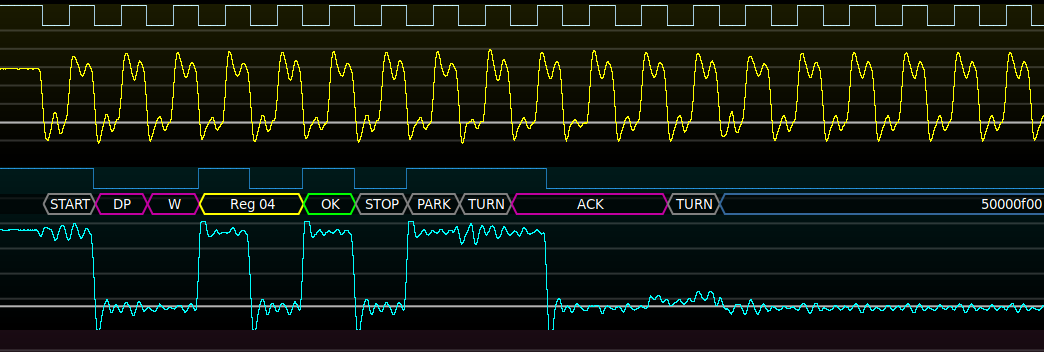
\includegraphics[width=16cm]{images/filters/swd.png}
\caption{Example of SWD protocol decode}
\label{swd_example}
\end{figure}

\subsection{Inputs}

\begin{tabularx}{16cm}{llX}
\thickhline
\textbf{Signal name} & \textbf{Type} & \textbf{Description} \\
\thickhline
SWDIO & Digital & Serial Wire Data In/Out (To/From target)\\
SWCLK & Digital & Serial Wire Clock In (To Target from Debug Probe)\\
\thickhline
\end{tabularx}

\subsection{Parameters}

No parameters are required for configuration of SWD. The protocol is clocked by SWCLK.

\subsection{Output Signal}

The SWD bus decode outputs a time series of SWD message elements, each of which may be one or a number of bits long.
Each message element consist of a type and optional numeric content.

\begin{tabularx}{16cm}{lllX}
\thickhline
\textbf{Type} & \textbf{Description} & \textbf{Color} & \textbf{Format} \\
\thickhline
Line Control & Line Reset & \cellcolor{preamble}\textcolor{white}{Preamble} & LINE RESET \\
\thickhline
Line Mode & Line Mode Change to SWD & \cellcolor{control}\textcolor{white}{Control} & JTAG TO SWD \\
\thickhline
Line Mode & Line Mode Change to JTAG & \cellcolor{control}\textcolor{white}{Control} & SWD TO JTAG \\
\thickhline
Line Mode & Line Mode Change to Dormant & \cellcolor{control}\textcolor{white}{Control} & SWD TO DORMANT \\
\thickhline
Line Mode & Leave Dormant Mode & \cellcolor{control}\textcolor{white}{Control} & LEAVE DORMANT \\
\thickhline
Start & Start of frame & \cellcolor{preamble}\textcolor{white}{Preamble} & START \\
\thickhline
APnDP & Selection between AP and DP & \cellcolor{control}\textcolor{white}{Control} & AP|DP  \\
\thickhline
RnW & Read or Write mode & \cellcolor{control}\textcolor{white}{Control} & R|W  \\
\thickhline
ADDR & AP or DP Address & \cellcolor{address}\textcolor{black}{Address} & Reg \%02x \\
\thickhline
Parity & Good Header Parity & \cellcolor{green}\textcolor{black}{Control} & OK  \\
\thickhline
Parity & Bad Header Parity & \cellcolor{red}\textcolor{white}{Control} & BAD  \\
\thickhline
Stop & End of Header & \cellcolor{preamble}\textcolor{white}{Preamble} & STOP \\
\thickhline
Park & Line Release & \cellcolor{preamble}\textcolor{white}{Preamble} & PARK \\
\thickhline
Turnaround & Line Direction Change & \cellcolor{preamble}\textcolor{white}{Preamble} & TURN \\
\thickhline
Acknowledge & Good Response from target to request & \cellcolor{control}\textcolor{white}{Control} & ACK|WAIT    \\
\thickhline
Acknowledge & Bad Response from target to request & \cellcolor{control}\textcolor{white}{Control} & FAULT|ERROR    \\
\thickhline
Data & Payload to/From Target & \cellcolor{data}\textcolor{white}{Data} & \%08x \\
\thickhline

\thickhline
\end{tabularx}

%%%%%%%%%%%%%%%%%%%%%%%%%%%%%%%%%%%%%%%%%%%%%%%%%%%%%%%%%%%%%%%%%%%%%%%%%%%%%%%%%%%%%%%%%%%%%%%%%%%%%%%%%%%%%%%%%%%%%%%%
\pagebreak
\section{SWD MEM-AP}

Converts SWD accesses to MEM-AP registers into memory read-write transactions.

Reference: ARM Debug Interface v5 Architecture Specification, chapter 8.

%%%%%%%%%%%%%%%%%%%%%%%%%%%%%%%%%%%%%%%%%%%%%%%%%%%%%%%%%%%%%%%%%%%%%%%%%%%%%%%%%%%%%%%%%%%%%%%%%%%%%%%%%%%%%%%%%%%%%%%%
\pagebreak
\section{Tachometer}

Converts pulses from a tachometer to shaft speed

%%%%%%%%%%%%%%%%%%%%%%%%%%%%%%%%%%%%%%%%%%%%%%%%%%%%%%%%%%%%%%%%%%%%%%%%%%%%%%%%%%%%%%%%%%%%%%%%%%%%%%%%%%%%%%%%%%%%%%%%
\pagebreak
\section{Tapped Delay Line}

Generic FIR filter with arbitrary tap values and delays. Can be used as-is for testing FIR filter coefficients
calculated by hand, but most commonly used as a base class for more specialized filters.

%%%%%%%%%%%%%%%%%%%%%%%%%%%%%%%%%%%%%%%%%%%%%%%%%%%%%%%%%%%%%%%%%%%%%%%%%%%%%%%%%%%%%%%%%%%%%%%%%%%%%%%%%%%%%%%%%%%%%%%%
\pagebreak
\section{TDR}

Converts a TDR waveform from volts to reflection coefficient or impedance.

%%%%%%%%%%%%%%%%%%%%%%%%%%%%%%%%%%%%%%%%%%%%%%%%%%%%%%%%%%%%%%%%%%%%%%%%%%%%%%%%%%%%%%%%%%%%%%%%%%%%%%%%%%%%%%%%%%%%%%%%
\pagebreak
\section{TDR Step De-Embed}

Given a waveform of a fast rising step, calculate the frequency response of a de-embedding network to convert the
measured waveform into an ideal unit step. The resulting data can be exported to a Touchstone file.

The calculated response is typically used as input to the de-embed filter and applied to a TDR/TDT waveform generated
with the same pulse generator. This correction allows for overshoot, ringing, and other artifacts on the pulse to be
removed from the TDR/TDT response.

It is important that the input contain a single rising edge, and is reasonably stable before and after the edge.
If multiple cycles of the test step, or falling edges, are present inaccurate results may be obtained.

NOTE: this filter is still under development and not suitable for general use.

%%%%%%%%%%%%%%%%%%%%%%%%%%%%%%%%%%%%%%%%%%%%%%%%%%%%%%%%%%%%%%%%%%%%%%%%%%%%%%%%%%%%%%%%%%%%%%%%%%%%%%%%%%%%%%%%%%%%%%%%
\pagebreak
\section{Threshold}

Converts an analog waveform to digital by thresholding at a constant level (no hysteresis).

\subsection{Inputs}

\begin{tabularx}{16cm}{llX}
\thickhline
\textbf{Signal name} & \textbf{Type} & \textbf{Description} \\
\thickhline
din & Analog & Input waveform \\
\thickhline
\end{tabularx}

\subsection{Parameters}

\begin{tabularx}{16cm}{llX}
\thickhline
\textbf{Parameter name} & \textbf{Type} & \textbf{Description} \\
\thickhline
Threshold & Float & Decision threshold \\
\thickhline
\end{tabularx}

\subsection{Output Signal}

This filter outputs an digital waveform with one sample for each sample in the input, which is true if the
corresponding input sample is above the threshold and false if less than or equal.

%%%%%%%%%%%%%%%%%%%%%%%%%%%%%%%%%%%%%%%%%%%%%%%%%%%%%%%%%%%%%%%%%%%%%%%%%%%%%%%%%%%%%%%%%%%%%%%%%%%%%%%%%%%%%%%%%%%%%%%%
\pagebreak
\section{TIE}

Calculates the time interval error of a data or clock signal with respect to an ideal ``golden" clock (typically
obtained from a CDR PLL).

%%%%%%%%%%%%%%%%%%%%%%%%%%%%%%%%%%%%%%%%%%%%%%%%%%%%%%%%%%%%%%%%%%%%%%%%%%%%%%%%%%%%%%%%%%%%%%%%%%%%%%%%%%%%%%%%%%%%%%%%
\pagebreak
\section{Top}

Calculates the top (logical one level) of each cycle in a digital waveform. It is most commonly used as an input to
statistics, to view the average top of the entire waveform.

\subsection{Inputs}

\begin{tabularx}{16cm}{llX}
\thickhline
\textbf{Signal name} & \textbf{Type} & \textbf{Description} \\
\thickhline
din & Analog & Input waveform \\
\thickhline
\end{tabularx}

\subsection{Parameters}

This filter takes no parameters.

\subsection{Output Signal}

This filter outputs an analog waveform with one sample for each group of logical ones in the input signal, containing
the average value of the one level.

%%%%%%%%%%%%%%%%%%%%%%%%%%%%%%%%%%%%%%%%%%%%%%%%%%%%%%%%%%%%%%%%%%%%%%%%%%%%%%%%%%%%%%%%%%%%%%%%%%%%%%%%%%%%%%%%%%%%%%%%
\pagebreak
\section{UART}

%%%%%%%%%%%%%%%%%%%%%%%%%%%%%%%%%%%%%%%%%%%%%%%%%%%%%%%%%%%%%%%%%%%%%%%%%%%%%%%%%%%%%%%%%%%%%%%%%%%%%%%%%%%%%%%%%%%%%%%%
\pagebreak
\section{USB 1.0 / 2.x Activity}

%%%%%%%%%%%%%%%%%%%%%%%%%%%%%%%%%%%%%%%%%%%%%%%%%%%%%%%%%%%%%%%%%%%%%%%%%%%%%%%%%%%%%%%%%%%%%%%%%%%%%%%%%%%%%%%%%%%%%%%%
\pagebreak
\section{USB 1.0 / 2.x Packet}

%%%%%%%%%%%%%%%%%%%%%%%%%%%%%%%%%%%%%%%%%%%%%%%%%%%%%%%%%%%%%%%%%%%%%%%%%%%%%%%%%%%%%%%%%%%%%%%%%%%%%%%%%%%%%%%%%%%%%%%%
\pagebreak
\section{USB 1.0 / 2.x PCS}

%%%%%%%%%%%%%%%%%%%%%%%%%%%%%%%%%%%%%%%%%%%%%%%%%%%%%%%%%%%%%%%%%%%%%%%%%%%%%%%%%%%%%%%%%%%%%%%%%%%%%%%%%%%%%%%%%%%%%%%%
\pagebreak
\section{USB 1.0 / 2.x PMA}

%%%%%%%%%%%%%%%%%%%%%%%%%%%%%%%%%%%%%%%%%%%%%%%%%%%%%%%%%%%%%%%%%%%%%%%%%%%%%%%%%%%%%%%%%%%%%%%%%%%%%%%%%%%%%%%%%%%%%%%%
\pagebreak
\section{Undershoot}

%%%%%%%%%%%%%%%%%%%%%%%%%%%%%%%%%%%%%%%%%%%%%%%%%%%%%%%%%%%%%%%%%%%%%%%%%%%%%%%%%%%%%%%%%%%%%%%%%%%%%%%%%%%%%%%%%%%%%%%%
\pagebreak
\section{Upsample}

Upsamples a waveform using sin(x)/x interpolation.

%%%%%%%%%%%%%%%%%%%%%%%%%%%%%%%%%%%%%%%%%%%%%%%%%%%%%%%%%%%%%%%%%%%%%%%%%%%%%%%%%%%%%%%%%%%%%%%%%%%%%%%%%%%%%%%%%%%%%%%%
\pagebreak
\section{Vertical Bathtub}

%%%%%%%%%%%%%%%%%%%%%%%%%%%%%%%%%%%%%%%%%%%%%%%%%%%%%%%%%%%%%%%%%%%%%%%%%%%%%%%%%%%%%%%%%%%%%%%%%%%%%%%%%%%%%%%%%%%%%%%%
\pagebreak
\section{Waterfall}

%%%%%%%%%%%%%%%%%%%%%%%%%%%%%%%%%%%%%%%%%%%%%%%%%%%%%%%%%%%%%%%%%%%%%%%%%%%%%%%%%%%%%%%%%%%%%%%%%%%%%%%%%%%%%%%%%%%%%%%%
\pagebreak
\section{Windowed Autocorrelation}

Calculates the cross-correlation between a fixed size block of the input signal and another block of the same size.

This will produce maximal response for a signal which has periodicity with the specified period and block size.

For example, period 4 and block size 2 will match aa**aa**.

This can be used to identify OFDM symbols.

\chapter{Internals}

\section{Introduction}

This chapter provides a high level overview of libscopehal and glscopeclient internals. It is intended for developers
to gain an understanding of the overall project architecture and how key pieces fit together, but is not a substitute
for the low level API documentation (Doxygen).

Many of the entities described below use a dynamic discovery / registration system. This allows all such classes to be
enumerated (and associated with human-readable names), and allows for objects of any registered type - including those
provided by plugins - to be created at run time by a factory method given the human-readable class name.

\section{Instruments}
\label{sec:instruments}

An instrument is an instance of a class derived from \codestyle{Instrument}, which represents an arbitrary piece of
laboratory equipment. As of this writing, an instrument may be an oscilloscope, multimeter, power supply, baseband
signal generator, or RF signal generator - or an arbitrary combination of these (for example an oscilloscope with
integrated function generator is both an oscilloscope and baseband signal generator).

The type of an instrument is defined by a bit field and may be queried by calling \codestyle{GetInstrumentTypes()}. Do
\emph{not} rely on C++ RTTI to determine the type of an instrument, for example it is incorrect to
\codestyle{dynamic\_cast} a \codestyle{Instrument*} pointer to \codestyle{Oscilloscope*} to check if the instrument is
an oscilloscope. This is because the C++ type of an object is fixed when the driver class is compiled, and the driver
may be used with many different instruments with various sets of software and hardware options. In other words, the
fact that a given driver supports \emph{some} device that contains multimeter functionality does not in any way imply
that the \emph{particular} device you are talking to is a multimeter.

The Instrument class provides no functionality other than describing the device (querying make/model/serial number,
assigning display nicknames, and querying feature set). To do any useful work, the object is normally casted to a
derived type to gain access to that device class's API.

\section{SCPI Devices}
\label{sec:scpidevices}

A SCPI device is an instance of a class derived from \codestyle{SCPIDevice}, which represents a device which speaks
some variant of SCPI. The vast majority of instrument driver classes derive from both \codestyle{SCPIDevice} and one or
more \codestyle{Instrument} derived classes.

A SCPI device object uses a \hyperref[sec:transports]{transport} to communicate with the associated instrument, which
avoids the need for the driver class to concern itself with the specifics of how the SCPI commands are transferred to
the device.

\section{Transports}
\label{sec:transports}

A transport is an instance of a class derived from \codestyle{SCPITransport}, which provides a means of sending SCPI
commands and/or raw byte string data to or from a physical instrument.

Most transports use a single stream in the underlying protocol layer (such as a single TCP socket) to transport both
control plane content (SCPI commands) and data plane content (waveform data), however some specialized protocols have
multiple physical streams (for example the \codestyle{SCPITwinLanTransport} transport). For these instruments, the
command/reply APIs and raw data APIs may not go to the same place.

All transports must be registered in order to be used by glscopeclient. To register a transport class, add the macro
\codestyle{TRANSPORT\_INITPROC(FooTransport)} to your class declaration and call
\codestyle{AddTransportClass(FooTransport)} in either the \texttt{TransportStaticInit} function within libscopehal or
the \codestyle{PluginInit} function of a plugin, as appropriate.

The special class \codestyle{SCPINullTransport} serves as a \texttt{/dev/null} equivalent: it discards anything written
to it, and never returns read data. It is primarily intended to be used by the ``demo" driver, which does not connect
to a real instrument.

While it is in principle possible to create a driver class that talks directly to a device via e.g. a USB API and
bypasses the transport model, this is strongly discouraged for user experience and flexibility reasons. Most drivers
for such devices (for example the Digilent and Pico drivers) instead consist of two components: a bridge server that
converts the instrument API to SCPI commands on one socket and a raw sample data on a second socket, and a
libscopehal-side driver that converts this to the relevant instrument API.

\section{Oscilloscopes}
\label{sec:oscilloscopes}

An Oscilloscope is an instance of a class derived from \codestyle{Oscilloscope}, which represents a device for
acquiring sampled digital data. All actual oscilloscopes use this API, as do some other instruments such as spectrum
analyzers. Most oscilloscope driver classes derive from \codestyle{SCPIOscilloscope} rather than directly from
\codestyle{Oscilloscope}, as they use SCPI to communicate with the hardware.

An oscilloscope may have zero or more \hyperref[sec:channels]{channels}. \footnote{All currently extant implementations
have at least one channel, however it is plausible that a zero-channel instrument might exist in the future (for
example, some sort of external trigger controller that exposes the same trigger API as a conventional oscilloscope) so
the API allows for this.}

At any given time, an oscilloscope has exactly one \hyperref[sec:triggers]{trigger} associated with it. A trigger has
inputs and properties just like a \hyperref[sec:filters]{filter}, since both are derived from
\codestyle{FlowGraphNode}. Most triggers take at least one input, however zero-input triggers are possible (for
example, triggering on AC mains zero crossings).

Every oscilloscope driver class must contain a public static method \codestyle{GetDriverNameInternal()}, which returns a
\codestyle{std::string} containing a short, human readable name for the driver (for example ``agilent" or ``pico"). By
convention, the driver name should consist of lowercase letters and numbers only - no spaces, punctuation, or capital
letters.

Just like transports, every oscilloscope driver class must be registered in the dynamic creation table by invoking
\codestyle{OSCILLOSCOPE\_INITPROC(MyOscilloscope)} in the class declaration and
\codestyle{AddDriverClass(MyOscilloscope)} in \texttt{DriverStaticInit} or \texttt{PluginInit}.

\section{Channels}
\label{sec:channels}

A channel is an instance of a class derived from \codestyle{OscilloscopeChannel}, which represents a single source of
data and associated controls. A channel may be associated with an \hyperref[sec:oscilloscopes]{oscilloscope}, or it may
be a \hyperref[sec:filters]{filter} which is not associated with any particular physical instrument.

Channels of an oscilloscope generally map 1:1 to analog front ends. Most commonly they are also 1:1 with instrument front
panel connectors, however there are some notable exceptions. Some high end oscilloscopes (such as the Teledyne LeCroy
WaveMaster family) have multiple inputs with a multiplexer feeding a single front end; this ensemble is considered to
be a single channel by libscopehal. Network analyzers have separate channels for receive and reflected power, for
example $S_{11}$ and $S_{12}$ of a VNA are measured at the same physical port on the instrument but separate channels
in libscopehal.

A channel normally has one or more output \hyperref[sec:streams]{streams}, however in some less common situations (such
as dedicated trigger inputs) there may be zero streams.

Channels are reference counted: when at least one filter or waveform view is consuming the output of a channel it will
be automatically enabled. When the last user of a channel is removed, the channel will be disabled and, if a filter,
deleted.

Various properties can be configured on channels, such as gain/offset and bandwidth limiters. Depending on whether the
channel is a filter or not, or what kind of oscillocope it is connected to, not all of these settings may be available.

\section{Streams}
\label{sec:streams}

A stream is an output from a \hyperref[sec:channels]{channel}. Most channels of physical oscilloscopes have only a
single stream, however some have multiple (for example I and Q from a realtime spectrum analyzer, or magnitude and
angle from a VNA). Many filters have multiple output streams, for example each channel of an imported WAV file is a
separate stream of the import filter.

All streams of a channel must have the same X axis unit, however they may have independent Y axis units.

The set of streams provided by a filter may change at run time, most commonly if an import filter is pointed to a new
file. When a filter changes its set of output streams, it must emit the \codestyle{m\_outputsChangedSignal} signal so
that other code can handle the change appropriately.

\section{Triggers}
\label{sec:triggers}

TODO: write this section

\section{Waveforms}
\label{sec:waveforms}

A waveform is a class derived from \codestyle{WaveformBase} which stores a vector of sampled data. The
\codestyle{AnalogWaveform} and \codestyle{DigitalWaveform} classes store 32-bit floating point and Boolean data
respectively. Additional waveform classes are defined by many protocol decodes to store data of arbitrary class type.

The units for X and Y axis are not specified in the waveform, but are properties of the channel / stream that the
waveform came from. Most commonly, for analog oscilloscope waveforms, the X axis unit is femtoseconds and the Y axis
unit is volts - but other units may be encountered, for example the output of a FFT has X axis units in Hz and Y axis
in dBm.\footnote{Some variables and methods throughout the project (especially in older code) use ``time" or
``voltage" terminology to refer to the current X or Y axis units. This will likely be changed through refactoring over
the long term.}

Waveforms store timestamp / header metadata as well as three vectors of data:

\begin{itemize}
\item \codestyle{m\_offsets}: start time of each sample
\item \codestyle{m\_durations}: length of each sample
\item \codestyle{m\_samples}: actual sample data
\end{itemize}

All three vectors must always be the same length. (The struct-of-arrays memory format allows for better cache locality
and is more SIMD-friendly than an array-of-structs format.)

Sample offsets and durations are measured in time base units (defined by \codestyle{m\_timescale}). This is commonly
the sample rate of the ADC or logic analyzer that acquired the data, however for upsampled or interpolated data smaller
time scale values - as low as 1 - may be used. A static offset, the ``trigger phase" (\codestyle{m\_triggerPhase}),
measured in raw X axis units and not scaled by \codestyle{m\_timescale}, is added to the timestamp of every signal
after scaling by the time base unit. This is commonly used to apply a sub-sample offset to a waveform for trigger
interpolation or de-skewing.

The final timestamp of sample \emph{i}, in X axis units, is thus \codestyle{m\_offsets[i]}*\codestyle{m\_timescale} +
\codestyle{m\_triggerPhase}.

Note that the offset/duration allows samples to have arbitrary length and spacing; i.e. waveforms are inherently
sparse. This is necessary to support protocol events, irregularly sampled data, etc. Sample timestamps must increase
monotonically: sample \emph{i+1} must start at or after the end of sample \emph{i}.

The majority of waveforms (such as those coming directly off an oscilloscope) will be uniformly sampled, which renders
the sparse storage format inefficient. A waveform of N samples which has a duration of 1 for every sample, and offsets
ranging from 0 to \emph{N-1}, is considered to be ``dense packed" and should have the \codestyle{m\_densePacked} flag
set to enable various processing optimizations. The dense pack flag must NOT be set on a waveform which does not meet
these criteria as this can lead to incorrect output.

Filters presented with input marked as dense packed are free to ignore the timestamp and duration flags at their input.
Filters generating densely packed output should set the dense pack flag, however they must still fill the timestamp and
duration vectors for use by filters which do not have an optimized special case for dense packed inputs.

\section{Filters}
\label{sec:filters}

TODO: write this section

\section{Plugins}

A plugin is a shared library which may contain transports, drivers, filters, and export wizards. All of these must be
registered in a function called \codestyle{PluginInit} exported with extern "C" linkage.

Plugins are automatically loaded at startup by glscopeclient, however standalone applications using libscopehal must
explicitly call \codestyle{InitializePlugins()} to load them.

\subsection{Linux}

On Linux, plugins are loaded from the following directories:

\begin{itemize}
\item \codestyle{/usr/lib/scopehal/plugins}
\item \codestyle{/usr/local/lib/scopehal/plugins}
\item \codestyle{~/.scopehal/plugins}
\item Executable directory, if not under \codestyle{/usr}
\end{itemize}

\subsection{Windows}

On Windows, plugins are loaded from the following directories:

\begin{itemize}
\item \codestyle{(Executable directory) \textbackslash plugins}
\end{itemize}


\end{document}
